\documentclass[english,,man,floatsintext]{apa6}
\usepackage{lmodern}
\usepackage{amssymb,amsmath}
\usepackage{ifxetex,ifluatex}
\usepackage{fixltx2e} % provides \textsubscript
\ifnum 0\ifxetex 1\fi\ifluatex 1\fi=0 % if pdftex
  \usepackage[T1]{fontenc}
  \usepackage[utf8]{inputenc}
\else % if luatex or xelatex
  \ifxetex
    \usepackage{mathspec}
  \else
    \usepackage{fontspec}
  \fi
  \defaultfontfeatures{Ligatures=TeX,Scale=MatchLowercase}
\fi
% use upquote if available, for straight quotes in verbatim environments
\IfFileExists{upquote.sty}{\usepackage{upquote}}{}
% use microtype if available
\IfFileExists{microtype.sty}{%
\usepackage{microtype}
\UseMicrotypeSet[protrusion]{basicmath} % disable protrusion for tt fonts
}{}
\usepackage{hyperref}
\hypersetup{unicode=true,
            pdftitle={How Optimal is Novel Word Recogntion Under Multimodal Uncertainty?},
            pdfauthor={Abdellah Fourtassi~\& Michael C. Frank},
            pdfkeywords={Language understanding; audio-visual processing; word learning; speech
perception; computational modeling.},
            pdfborder={0 0 0},
            breaklinks=true}
\urlstyle{same}  % don't use monospace font for urls
\ifnum 0\ifxetex 1\fi\ifluatex 1\fi=0 % if pdftex
  \usepackage[shorthands=off,main=english]{babel}
\else
  \usepackage{polyglossia}
  \setmainlanguage[]{english}
\fi
\usepackage{graphicx,grffile}
\makeatletter
\def\maxwidth{\ifdim\Gin@nat@width>\linewidth\linewidth\else\Gin@nat@width\fi}
\def\maxheight{\ifdim\Gin@nat@height>\textheight\textheight\else\Gin@nat@height\fi}
\makeatother
% Scale images if necessary, so that they will not overflow the page
% margins by default, and it is still possible to overwrite the defaults
% using explicit options in \includegraphics[width, height, ...]{}
\setkeys{Gin}{width=\maxwidth,height=\maxheight,keepaspectratio}
\IfFileExists{parskip.sty}{%
\usepackage{parskip}
}{% else
\setlength{\parindent}{0pt}
\setlength{\parskip}{6pt plus 2pt minus 1pt}
}
\setlength{\emergencystretch}{3em}  % prevent overfull lines
\providecommand{\tightlist}{%
  \setlength{\itemsep}{0pt}\setlength{\parskip}{0pt}}
\setcounter{secnumdepth}{0}
% Redefines (sub)paragraphs to behave more like sections
\ifx\paragraph\undefined\else
\let\oldparagraph\paragraph
\renewcommand{\paragraph}[1]{\oldparagraph{#1}\mbox{}}
\fi
\ifx\subparagraph\undefined\else
\let\oldsubparagraph\subparagraph
\renewcommand{\subparagraph}[1]{\oldsubparagraph{#1}\mbox{}}
\fi

%%% Use protect on footnotes to avoid problems with footnotes in titles
\let\rmarkdownfootnote\footnote%
\def\footnote{\protect\rmarkdownfootnote}


  \title{How Optimal is Novel Word Recogntion Under Multimodal Uncertainty?}
    \author{Abdellah Fourtassi\textsuperscript{1}~\& Michael C.
Frank\textsuperscript{1}}
    \date{}
  
\shorttitle{Word Identification Under Multimodal Uncertainty}
\affiliation{
\vspace{0.5cm}
\textsuperscript{1} Department of Psychology, Stanford University}
\keywords{Language understanding; audio-visual processing; word learning; speech perception; computational modeling.}
\usepackage{csquotes}
\usepackage{upgreek}
\captionsetup{font=singlespacing,justification=justified}

\usepackage{longtable}
\usepackage{lscape}
\usepackage{multirow}
\usepackage{tabularx}
\usepackage[flushleft]{threeparttable}
\usepackage{threeparttablex}

\newenvironment{lltable}{\begin{landscape}\begin{center}\begin{ThreePartTable}}{\end{ThreePartTable}\end{center}\end{landscape}}

\makeatletter
\newcommand\LastLTentrywidth{1em}
\newlength\longtablewidth
\setlength{\longtablewidth}{1in}
\newcommand{\getlongtablewidth}{\begingroup \ifcsname LT@\roman{LT@tables}\endcsname \global\longtablewidth=0pt \renewcommand{\LT@entry}[2]{\global\advance\longtablewidth by ##2\relax\gdef\LastLTentrywidth{##2}}\@nameuse{LT@\roman{LT@tables}} \fi \endgroup}


\usepackage{lineno}

\linenumbers
\usepackage[sortcites=false,sorting=none]{biblatex}

\authornote{ Abdellah Fourtassi

Department of Psychology

Stanford University

50 Serra Mall

Jordan Hall, Building 420

Stanford, CA 94301

Correspondence concerning this article should be addressed to Abdellah
Fourtassi, Postal address. E-mail:
\href{mailto:afourtas@stanford.edu}{\nolinkurl{afourtas@stanford.edu}}}

\abstract{
Identifying a spoken word in a referential context requires both the
ability to integrate multimodal input and the ability to reason under
uncertainty. How do these tasks interact with one another? We introduce
a paradigm that allows us to examine how adults identify novel words
under joint uncertainty in the auditory and visual modalities and
propose an ideal observer model of how cues in these modalities are
combined optimally. Model predictions are tested in three experiments
where novel word recognition is made under two kinds of uncertainty:
category ambiguity and perceptual noise. In all cases, the optimal model
explains much of the variance in human mean judgments. When the signal
is not distorted with noise, participants weight the auditory and visual
cues optimally, that is, according to the relative reliability of each
modality. But when one modality has noise added to it, human perceivers
systematically prefer the unperturbed modality to a greater extent than
the optimal model does. The study provides a formal framework which
helps to quantify how word form and word meaning interact in word
recognition under uncertainty. Moreover it offers a first step towards a
model that accounts for form-meaning synergies in early word learning.


}

\usepackage{amsthm}
\newtheorem{theorem}{Theorem}[section]
\newtheorem{lemma}{Lemma}[section]
\theoremstyle{definition}
\newtheorem{definition}{Definition}[section]
\newtheorem{corollary}{Corollary}[section]
\newtheorem{proposition}{Proposition}[section]
\theoremstyle{definition}
\newtheorem{example}{Example}[section]
\theoremstyle{definition}
\newtheorem{exercise}{Exercise}[section]
\theoremstyle{remark}
\newtheorem*{remark}{Remark}
\newtheorem*{solution}{Solution}
\begin{document}
\maketitle

\begin{verbatim}
## Warning: package 'bindrcpp' was built under R version 3.4.4
\end{verbatim}

\section{Introduction}\label{introduction}

Language uses symbols expressed in one modality -- the auditory
modality, in the case of speech -- to communicate about the world, which
we perceive through many different sensory modalities. Consider hearing
someone yell \enquote{bee!} at a picnic, as a honey bee buzzes around
the food. Identifying a word involves processing the auditory
information as well as other perceptual signals (e.g., the visual image
of the bee, the sound of its wings, the sensation of the bee flying by
your arm). A word is successfully identified when information from these
modalities provide convergent evidence. However, word identification
takes place in a noisy world, and the cues received through each
modality may not provide a definitive answer. On the auditory side,
individual acoustic word tokens are almost always ambiguous with respect
to the particular sequence of phonemes they represent, which is due to
the inherent variability of how a phonetic category is realized
acoustically (Hillenbrand, Getty, Clark, \& Wheeler, 1995). And some
tokens may be distorted additionally by mispronunciation or ambient
noise. Perhaps the speaker was yelling \enquote{pea} and not
\enquote{bee.} Similarly, a sensory impression may not be enough to make
a definitive identification of a visual
category.\footnote{In the general case, language can of course be visual as well as auditory, and object identification can be done through many modalities. For simplicity, we focus on audio-visual matching here.}
Perhaps the insect was a beetle or a fly instead. How does the listener
deal with such multimodal uncertainty to recognize the speaker's
intended word?

As a simplified case study of early word learning, the task of matching
sounds to corresponding visual objects has been studied extensively in
the developmental literature. For example, many studies focus on how
children might succeed in this type of task despite referential
ambiguity (Medina, Snedeker, Trueswell, \& Gleitman, 2011; Pinker, 1989;
Smith \& Yu, 2008; Suanda, Mugwanya, \& Namy, 2014; Vlach \& Johnson,
2013; Vouloumanos, 2008; Yurovsky \& Frank, 2015). However, even when
they \emph{know} the meanings of a word, listeners (both children and
adults) often still find it challenging to recognize which word the
speaker has uttered, especially under noise (Mattys, Davis, Bradlow, \&
Scott, 2012; Peelle, 2018). The purpose of the current study is thus to
explore word recognition by adults under multimodal uncertainty. We
focus on the special case where people have access to multimodal cues
from the auditory speech and the visual referent. In the General
Discussion, we return to the question of how these findings relate to
questions about word learning.

One rigorous way to approach this question is through conducting an
\emph{ideal observer} analysis. This research strategy provides a
characterization of the task/goal and shows what the optimal performance
should be under this characterization.\footnote{It is, thus, a general
  instance of the rational approach to cognition (Anderson, 1990),
  instantiating Marr's computational level of analysis (Marr, 1982).}
When there is uncertainty in the input, the ideal observer performs an
optimal probabilistic inference. For example, in order to recognize an
ambiguous linguistic input, the model uses all available probabilistic
knowledge in order to maximize the accuracy of this recognition. The
ideal observer model can be seen as a theoretical upper limit on
performance. It is not so much a realistic model of human performance,
as much as a baseline against which human performance can be compared
(Geisler, 2003; Rahnev \& Denison, 2018). When there is a deviation from
the ideal, it can reveal extra constraints on human cognition, such as
limitations on the working memory or attentional resources. This
approach has had a tremendous impact not only on speech-related research
(Clayards, Tanenhaus, Aslin, \& Jacobs, 2008; Feldman, Griffiths, \&
Morgan, 2009; Kleinschmidt \& Jaeger, 2015; Norris \& McQueen, 2008),
but also on many other disciplines in the cognitive sciences (for
reviews, see Chater \& Manning, 2006; Knill \& Pouget, 2004; Tenenbaum,
Kemp, Griffiths, \& Goodman, 2011)

Some prior ideal observer studies are closely related to the question we
are addressing in the current work. For instance, Clayards et al. (2008)
simulated auditory uncertainty by manipulating the probability
distribution of a cue (Voice Onset Time) that differentiated similar
words (e.g., \enquote{beach} and \enquote{peach}). They found that
humans were sensitive to these probabilistic cues and their judgments
closely reflected the optimal predictions. And Feldman et al. (2009)
studied the perceptual magnet effect, a phenomenon that involves reduced
discriminability near prototypical sounds in the native language (Kuhl,
1991), showing that this effect can be explained as the consequence of
optimally solving the problem of perception under uncertainty.

Besides the acoustic cues explored in Clayards et al. (2008) and Feldman
et al. (2009), there is extensive evidence that information from the
visual modality, such as the speaker's facial features, also influences
speech understanding (see Campbell, 2008 for a review). Bejjanki,
Clayards, Knill, and Aslin (2011) offered a mathematical
characterization of how probabilistic cues from speech and lip movements
can be optimally combined. They showed that human performance during
audio-visual phonemic labeling was consistent (at least at the
qualitative level) with the predictions of an ideal observer. This
previous research did not, however, systematically study speech
understanding when visual information was obtained through the
referential context rather than through observation of speaker's face.
Although some experimental findings show that information about the
identity of a referent can be integrated with linguistic information to
resolve lexical and syntactic ambiguities in speech (e.g., Eberhard,
Spivey-Knowlton, Sedivy, \& Tanenhaus, 1995; Spivey, Tanenhaus,
Eberhard, \& Sedivy, 2002; Tanenhaus, Spivey-Knowlton, Eberhard, \&
Sedivy, 1995), to our knowledge no study has offered an ideal observer
analysis of this task.

Combining information between words and visual referents might seem
similar to audio-visual speech integration, but there are at least two
fundamental differences between these two cases, and both can influence
the way the auditory and visual cues are combined.

First, in the case of audio-visual speech, both modalities offer
information about the same underlying speech category. They differ only
in terms of their informational reliability. In a referential context,
however, the auditory and visual modalities play different roles in the
referential process -- the auditory input represents the \emph{symbol}
whereas the visual input represents the \emph{meaning} (and these
differences are in addition to possible differences in informational
reliability). Further, speech is claimed to have a privileged status
compared to other sensory stimuli (Edmiston \& Lupyan, 2015; Lupyan \&
Thompson-Schill, 2012; Vouloumanos \& Waxman, 2014; Waxman \& Gelman,
2009; Waxman \& Markow, 1995), and that this privilege is suggested to
be specifically related to the ability to refer (Waxman \& Gelman,
2009).\footnote{There is, however, a debate as to whether speech is
  privileged for children and adults for similar reasons. Whereas some
  researchers suggest that speech is privileged for both children and
  adults because of its ability to refer (e.g., Waxman \& Gelman, 2009),
  others suggest that speech might \emph{not} have a referential status
  from the start. Rather, speech might be preferred by children only
  because of a low level auditory ``overshadowing'' (e.g., Sloutsky \&
  Napolitano, 2003).} Thus, in a referential context, it is possible
that listeners do not treat the auditory and visual modalities as
equivalent sources of information. Instead, there could be a sub-optimal
bias for the auditory modality beyond what is expected from
informational reliability alone.

Second, in the case of audio-visual speech, the auditory and visual
stimuli are expected to be perceptually correlated. The expectation for
this correlation is strong enough that when there is a mismatch between
the auditory and visual input, they are still integrated into a unified
(but illusory) percept (e.g., the McGurk Effect; McGurk \& MacDonald,
1976). In the case of referential language, however, the multimodal
association is by nature \emph{arbitrary} (Greenberg, 1957; Saussure,
1916). For instance, there is no logical or perceptual connection
between the sound \enquote{bee} and the corresponding insect. Moreover,
variation in the way the sound \enquote{bee} is pronounced is generally
not expected to correlate perceptually with variation in the shape (or
any other visual property) in the category of bees. In sum, cue
combination in the case of arbitrary audio-visual associations
(word-referent) is likely to be less automatic, more effortful, and
therefore less conducive to optimal integration than it is in the case
of perceptually correlated associations (as in audio-visual speech
perception).

\subsection{The current study}\label{the-current-study}

We investigate how cues from the auditory and the visual modality are
combined in recognizing words in a referential context. In particular,
we study how this combination is performed under various degrees of
uncertainty in both the auditory and the visual modality. Imagine, for
example, that someone is uncertain whether they heard \enquote{pea} or
\enquote{bee.} Does this uncertainty make them rely more on the referent
(e.g., the object being pointed at)? Or, if they are not sure if they
saw a bee or a fly, does this uncertainty make them rely more on the
sound? More importantly, when input in both modalities is uncertain to
varying degrees, do they weight each modality according to its relative
reliability (the optimal strategy), or do they over-rely on a particular
modality?

We begin by proposing an ideal observer model that performs the
combination in an optimal fashion. We then compare the predictions of
the optimal model to human responses. Humans can deviate from the ideal
for several reasons. For instance, as mentioned above, a sub-optimality
can be induced by the privileged status of a particular modality or by
the arbitrariness of the referential association. In order to study
possible patterns of sub-optimality, we compare the optimal model (which
provides a normative benchmark) to a descriptive model (which is fit to
human responses). Comparing parameter estimates between these two
formulations allows us to quantify the degree of deviation from
optimality.

We tested the ideal observer model's predictions in three behavioral
experiments where we varied the source of uncertainty. In Experiment 1,
audio-visual tokens were ambiguous with respect to their category
membership only. In Experiment 2, we intervened by adding perceptual
noise to the auditory modality, and in Experiment 3, we intervened by
adding perceptual noise to the visual modality. In all experiments,
participants were quantitatively near-optimal, though overall response
precision was slightly lower than expected. In Experiment 1 -- where
neither of the modalities was perturbed with background noise --
participants weighted auditory and visual cues according to the relative
reliability predicted by the optimal model. However, in Experiment 2 and
3, participants over-relied on one modality when the other modality was
perturbed with additional noise.

\section{Paradigm and Models}\label{paradigm-and-models}

In this section we first briefly introduce the multimodal combination
task. Then we explain how behavior in this paradigm can be characterized
optimally with an ideal observer model.

\subsection{The Audio-Visual Word Recognition
Task}\label{the-audio-visual-word-recognition-task}

We introduce a paradigm adapted from a task used by Sloutsky and
Napolitano (2003). The original was used with both children and adults
to probe audio-visual encoding (see Robinson \& Sloutsky, 2010 for
review). Here we use a slightly different version to test word
recognition in a referential context. We use two visual categories (cat
and dog) and two auditory categories (/b/ and /d/ embedded in the
minimal pair /aba/-/ada/). For each participant, an arbitrary pairing is
set between the auditory and the visual categories, leading to two
audio-visual word categories (e.g., dog-/aba/, cat-/ada/). In each
trial, participants are presented with an audio-visual target (the
prototype of the target category), immediately followed by an
audio-visual test stimulus (Figure~\ref{fig:task}). The test stimulus
may differ from the target in both the auditory and the visual
components. After these two presentations, participants press
\enquote{same} or \enquote{different.}

\begin{figure}

{\centering 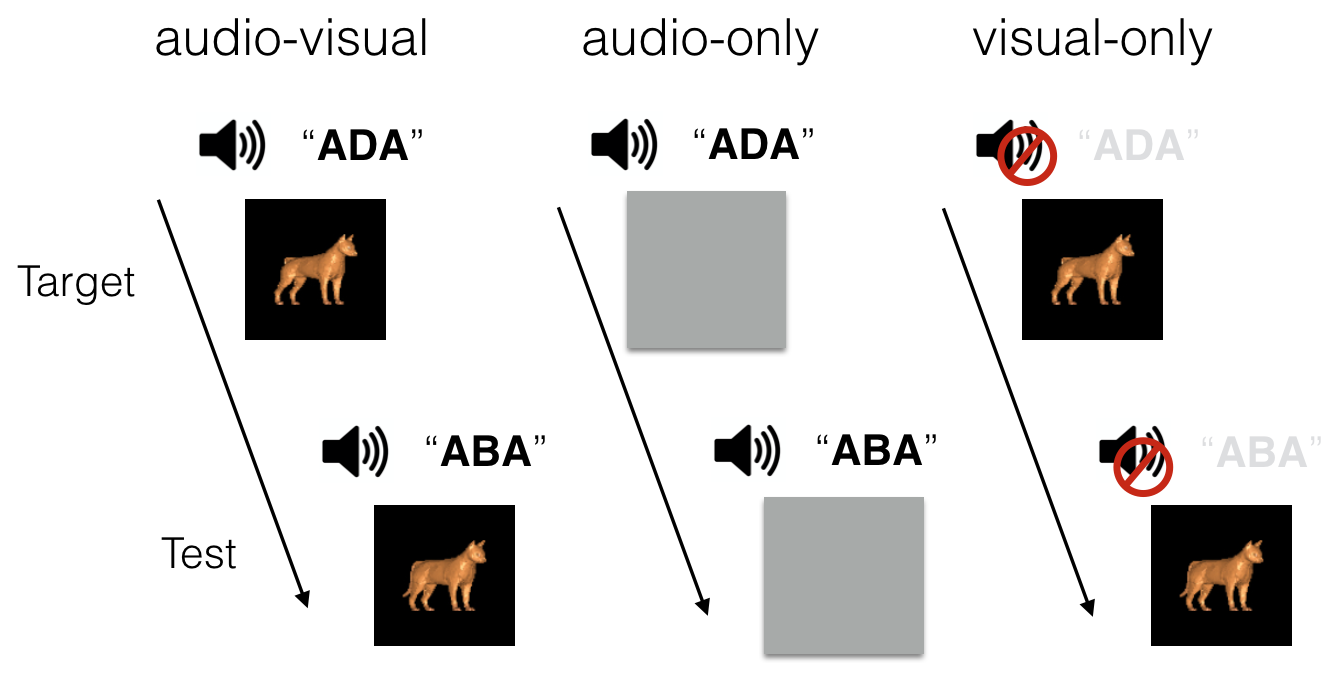
\includegraphics[width=400px]{pictures/task} 

}

\caption{Overview of the task. In the audio-visual condition, participants are first presented with an audio-visual target (the prototype of the target category), immediately followed by an audio-visual test. The test may differ from the target in both the auditory and the visual components. After these two presentations, participants press `same' (i.e., the same category as the target) or `different' (not the same category). The auditory-only and visual-only conditions are similar to the audio-visual condition, except that only the sounds are heard, or only the pictures are shown, respectively.}\label{fig:task}
\end{figure}

In the testing phase of the original task (Sloutsky \& Napolitano,
2003), participants were asked whether or not the two audio-visual
presentations are \emph{identical}. In the current study, we are
interested, rather, in the categorization, i.e., determining whether or
not two similar tokens are members of the same phonological/semantic
category. Therefore, testing in our task is category-based: Participants
are asked to press \enquote{same} if they think the second item (the
test) belongs to the same category as the first (target) (e.g.,
dog-/aba/), even if there is a slight difference in the sound, in the
referent, or in both. They are instructed to press \enquote{different}
only if they think that the second stimulus was an instance of the other
category (cat-/ada/). The task also includes trials where pictures are
hidden (audio-only) or where sounds are muted (visual-only). These
unimodal trials provide us with the participants' evaluation of the
probabilistic information present in the auditory and visual categories.
As we shall see, these unimodal distributions are used as inputs to the
optimal cue combination model.

\subsection{Optimal Model}\label{optimal-model}

We construct an ideal observer model that combines probabilistic
information from the auditory and visual modalities. In contrast to the
model used in most research on multisensory integration (e.g., Ernst \&
Banks, 2002), which typically studies continuous stimuli (e.g., size,
location), the probabilistic information in our case cannot be
characterized with \emph{sensory noise} only. Since our task involves
responses over categorical variables (phonemes and concepts), the
optimal model should take into account not only the noise variability
around an individual perceptual estimate but also its \emph{categorical
variability}, i.e., the uncertainty related to whether this perceptual
estimate belongs to a given category (see also Bankieris, Bejjanki, \&
Aslin, 2017; Bejjanki et al., 2011). In what follows, we describe a
model that accounts for both types of variability. First, we describe
the model in the simplified case of categorical variability only.
Second, we augment this simplified model to account for sensory noise.

\subsubsection{Categorical variability}\label{categorical-variability}

We assume that both the auditory categories (i.e., /aba/ and /ada/) and
the visual categories (cat and dog) are distributed along a single
acoustic and semantic dimension, respectively (Figure~\ref{fig:model}).
Moreover, we assume that all categories are normally distributed.
Formally speaking, if \(A\) denotes an auditory category (/ada/ or
/aba/), then the probability that a point \(a\) along the acoustic
dimension belongs to the category \(A\) is
\[ p(a | A) \sim  N(\mu_A, \sigma^2_A) \] where \(\mu_A\) and
\(\sigma^2_A\) are respectively the mean and the variance of the
auditory category. Similarly, the probability that a point \(v\) along
the visual dimension belongs to the category \(V\) is
\[ p(v | V) \sim  N(\mu_V, \sigma^2_V) \] where \(\mu_V\) and
\(\sigma^2_V\) are the mean and the variance of the visual category. An
audio-visual signal \(w=(a,v)\) can be represented as a point in the
audio-visual space. These audio-visual tokens define bivariate
distributions in the bi-dimentional space. We call these bivariate
distributions \emph{Word categories}, noted \(W\), and are distributed
as follows: \[ p(w | W) \sim  N(M_W, \Sigma_W) \] where
\(M_W=(\mu_A, \mu_V)\) and \(\Sigma_W\) are the mean and the covariance
matrix of the word category. The main assumption of the model is that
the auditory and visual variables are independent (i.e., uncorrelated),
so the covariance matrix is simply: \[
   \Sigma_W=
  \left[ {\begin{array}{cc}
   \sigma^2_A & 0 \\
   0 & \sigma^2_V \\
  \end{array} } \right]
\]

\begin{figure}[!h]
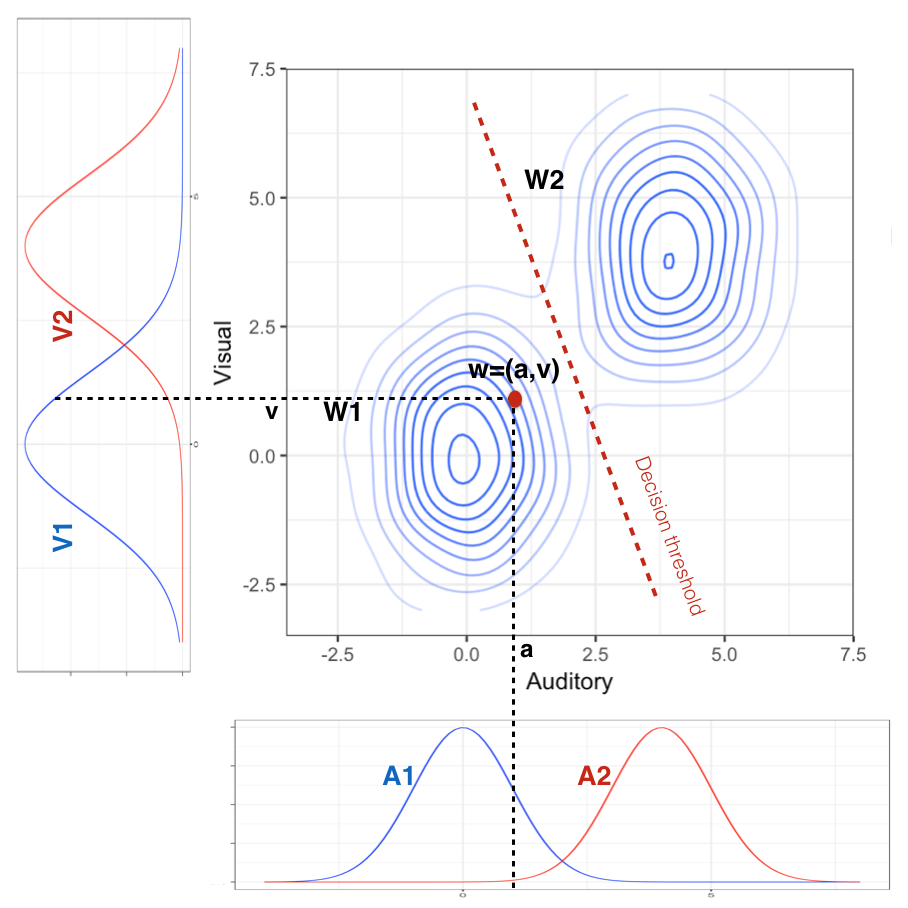
\includegraphics[width=\textwidth]{pictures/model} \caption{Illustration of the model using simulated data. A word category is defined as the joint bivariate distribution of an auditory category (horizontal, bottom panel) and a visual semantic category (vertical, left panel). Upon the presentation of a word token $w$, participants guess whether it is sampled from the word type $W_1$ or from the word type $W_2$. Decision threshold is where the guessing probability is 0.5.}\label{fig:model}
\end{figure}

\noindent This assumption says that, given a word-object mapping, e.g.,
\(W=\)(\enquote{cat}-CAT), variation in the way \enquote{cat} is
pronounced does not correlate with changes in any visual property of the
object CAT, which is a valid assumption in the context of our
task.\footnote{Note that this assumptions is more adequate in the case of arbitrary associations such as ours, and less so in the case of redundant association such as audio-visual speech. In the latter, variation in the pronunciation is expected to correlate, at least to some extent, with lip movements.}

Now we turn to the crucial question of modeling how the optimal decision
should proceed given the probabilistic (categorical) information in the
auditory and the visual modalities, as characterized above. We have two
word categories: dog-/aba/ (\(W_1\)) and cat-/ada/
(\(W_2\)).\footnote{This mapping is randomized in the experiments.} When
making decisions, participants can be understood as choosing one of
these two word categories (Figure~\ref{fig:model}). For an ideal
observer, the probability of choosing category 2 when presented with an
audio-visual instance \(w=(a,v)\) is the posterior probability of this
category: \[
p(W_2 | w)=\frac{p(w|W_2)p(W_2)}{p(w|W_2)p(W_2)+p(w|W_1)p(W_1)}
\] Using our assumption that the cues are uncorrelated, we have:
\[p(w | W) = p(a,v| W) = p(a| A)p(v| V)\] Under this assumption, the
posterior probability reduces to the following formula (see Appendix 1
for the details of the derivation):

\begin{equation}
 p(W_2 | w)=\frac{1}{1+(1+b)\exp(\beta_0+\beta_aa+\beta_vv)}
\end{equation}

where \[1+b=\frac{p(W_1)}{p(W_2)}\]
\[\beta_0=\frac{\mu^2_{A2}-\mu^2_{A1}}{2\sigma^2_{A}}+\frac{\mu^2_{V2}-\mu^2_{V1}}{2\sigma^2_{V}}\]

\[\beta_a=\frac{\mu_{A1}-\mu_{A2}}{\sigma^2_{A}}\]
\[\beta_v=\frac{\mu_{V1}-\mu_{V2}}{\sigma^2_{V}}.\]

The parameter \(b\) represents the differential between the categories'
prior probabilities. However, since the identity of word categories is
randomized across participants, \(b\) measures, rather, a response bias
to \enquote{same} if \(b > 0\), and a response bias to
\enquote{different} if \(b < 0\). We expect a general bias towards
answering \enquote{different} because of the categorical nature of our
same-different task: When two items are ambiguous but perceptually
different, participants might have a slight preference for
\enquote{different} over \enquote{same}. As for the means, their values
are fixed, and they correspond to the most typical tokens in our
stimuli. Finally, observations from each modality (\(a\) and \(v\)) are
weighted in Equation 1 according to their reliability (that is,
according to the \emph{inverse} of their variance):
\[\beta_a \propto \frac{1}{\sigma^2_{A}}\]
\[\beta_v \propto \frac{1}{\sigma^2_{V}}.\]

\subsubsection{Sensory variability}\label{sensory-variability}

So far, we have only accounted for categorical variability, i.e.,
\(\sigma^2_{A} = \sigma^2_{A_C}\). For instance, if the speaker
generates a target production \(a_t\) from an auditory category
\(p(a_t | A) \sim N(\mu_{A}, \sigma^2_{A_C})\), the ideal model assumes
that it has direct access to this production token (i.e., \(a=a_t\)),
and that all uncertainty is about the category membership of this token.
However, we might also want to account for internal noise in the brain
and/or external noise in the environment. For example, the observer
might not have access to the exact produced target, but only to the
target perturbed by noise. If we assume this noise to be normally
distributed, that is, \(p(a | a_t) \sim N(a_t, \sigma^2_{A_N})\), then
integrating over \(a_t\) leads to this new expression of the probability
distribution:
\[ p(a | A) \sim N(\mu_{A}, \sigma^2_{A_C}+\sigma^2_{A_N})\] Similarly,
in the case of sensory noise in the visual modality, we get:
\[ p(a | V) \sim N(\mu_{V}, \sigma^2_{V}+\sigma^2_{V_N})\] Finally,
using exactly the same derivation as above, we end up with the following
multimodal weighting scheme in the optimal combination model (Equation
1) which takes into account both categorical and sensory variability:

\[\beta_a \propto \frac{1}{\sigma^2_{A_C}+\sigma^2_{A_N}}\]
\[\beta_v \propto \frac{1}{\sigma^2_{V_C} +\sigma^2_{V_N}}.\]

\subsubsection{Optimal cue combination}\label{optimal-cue-combination}

Equation 1 provides the optimal model's predictions for how
probabilities that characterize uncertainty in the auditory and the
visual modalities can be combined to make categorical decisions.
Parameter estimates of the probability distributions in each modality
are derived by fitting unimodal posteriors to the participants'
responses in the unimodal conditions, i.e., the condition where only the
sounds are heard or only the pictures are seen
(Figure~\ref{fig:task}).\footnote{Further technical detail about model fitting in the unimodal conditions will be given in the method section of Experiment 1.}
Using these derived parameters, the optimal model makes predictions
about responses in the bimodal (i.e., audio-visual) condition where
participants both hear the sounds and see the pictures.

\subsubsection{Auditory and Visual
baselines}\label{auditory-and-visual-baselines}

The predictions of the optimal model will be compared to two baselines.
The first baseline is a visual model which assumes that participants
rely only on visual information, and an auditory model, which assumes
that participants rely only on auditory information. More precisely,
these baseline models assume that the participants' responses in the
bimodal condition will not be different from their response in either
the visual-only or the auditory-only condition. However, if the
participants rely on both the auditory and the visual modalities to make
decision in the bimodal condition, the optimal model would explain more
variance in human responses than the visual or the auditory model do.

\subsection{Descriptive model and analysis of
(sub-)optimality}\label{descriptive-model-and-analysis-of-sub-optimality}

The optimal model (as well as the auditory and visual baselines) are
\emph{normative} models. Their predictions are made about human data in
the bimodal condition, but their crucial parameters (i.e., variances
associated with the visual and auditory modalities) are derived from
data in the unimodal conditions. In addition to these normative models,
we consider a \emph{descriptive} model. It is formally identical to the
normative optimal model (Equation 1), except that the parameters are fit
to actual responses in the bimodal condition. If the referential task
induces sub-optimality (due, for instance, to the arbitrary nature of
the sound-object association), then the descriptive model should explain
more variance than the optimal model does.

Comparison of the optimal and the descriptive models allows us, not only
to quantify how much people deviate from optimality, but also to
understand precisely the nature of this deviation. Let \(\sigma^2_{A}\)
and \(\sigma^2_{V}\) be the values of the variances used in the optimal
model (derived from the unimodal conditions), and \(\sigma^2_{Ab}\) and
\(\sigma^2_{Vb}\) be the values observed through the descriptive model
in the bimodal condition. Deviation from optimality is measured in two
ways. First, we measure the change in the values of the variance
specific to each modality, that is, how \(\sigma^2_{A}\) compares to
\(\sigma^2_{Ab}\), and how \(\sigma^2_{V}\) compares to
\(\sigma^2_{Vb}\). Second, we measure changes in the proportion of the
visual and auditory variances, i.e., we examine how
\(\frac{\sigma^2_{A}}{\sigma^2_{V}}\) compares to
\(\frac{\sigma^2_{Ab}}{\sigma^2_{Vb}}\). The first measure allows us to
test if response precision changes for each modality when we move from
the unimodal to the bimodal conditions. The second allows us to test the
extent to which the weighting scheme follows the prediction of the
optimal model. The reason we used the proportion of the variances as a
measure of cross-modal weighting is because this proportion corresponds
to the
slope\footnote{Or more precisely the absolute value of the slope.} of
the decision threshold in the audio-visual space
(Figure~\ref{fig:model}). The decision threshold is defined as the set
of values in this audio-visual space along which the posterior is equal
to 0.5. Formally speaking, the decision threshold has the following
form:

\[v=-\frac{\sigma^2_V}{\sigma^2_A}a+v_0\]

If the absolute value of the slope derived from the descriptive model is
greater than that of the optimal model, the corresponding shift in the
decision threshold indicates that participants have a preference for the
auditory modality in the bimodal case. Similarly, a smaller absolute
value of the slope would lead to a preference for the visual modality.
The limit cases are when there is exclusive reliance on the auditory cue
(a vertical line), and where there is exclusive reliance on the visual
(a horizontal line).

There are three possible ways human responses can deviate from
optimality. These scenarios are illustrated in
Figure~\ref{fig:subOptim}, and are as follows:

\begin{enumerate}
\def\labelenumi{\arabic{enumi})}
\item
  Both variances may increase, but their proportion remains the same.
  That is, \(\sigma^2_{Ab} \geqslant \sigma^2_{A}\) and
  \(\sigma^2_{Vb} \geqslant \sigma^2_{V}\), but
  \(\frac{\sigma^2_{Ab}}{\sigma^2_{Vb}} \approx \frac{\sigma^2_{A}}{\sigma^2_{V}}\).
  In this case, sub-optimality would be due to increased randomness in
  human responses in the bimodal condition. However, this randomness
  would not affect the relative weighting of both modalities, i.e.,
  participants would still weigh modalities according to the relative
  reliability predicted by the optimal model.
\item
  The auditory variance increases at a higher rate. That is,
  \(\sigma^2_{Ab} \gg \sigma^2_{A}\) and
  \(\sigma^2_{Vb} \geqslant \sigma^2_{V}\), leading to
  \(\frac{\sigma^2_{Ab}}{\sigma^2_{Vb}} > \frac{\sigma^2_{A}}{\sigma^2_{V}}\).
  In this case, sub-optimality would consist not only in participants
  being more random in the bimodal condition, but also in having a
  systematic preference for the visual modality, even after accounting
  for informational reliability.
\item
  The visual variance increases at a higher rate. That is,
  \(\sigma^2_{Vb} \gg \sigma^2_{V}\), and
  \(\sigma^2_{Ab} \geqslant \sigma^2_{A}\), leading to
  \(\frac{\sigma^2_{Ab}}{\sigma^2_{Vb}} > \frac{\sigma^2_{A}}{\sigma^2_{V}}\).
  This case is the reverse of case 2, i.e., in addition to increased
  randomness in the bimodal condition, there is a systematic preference
  for the auditory modality, even after accounting for informational
  reliability.
\end{enumerate}

\begin{figure}[!h]
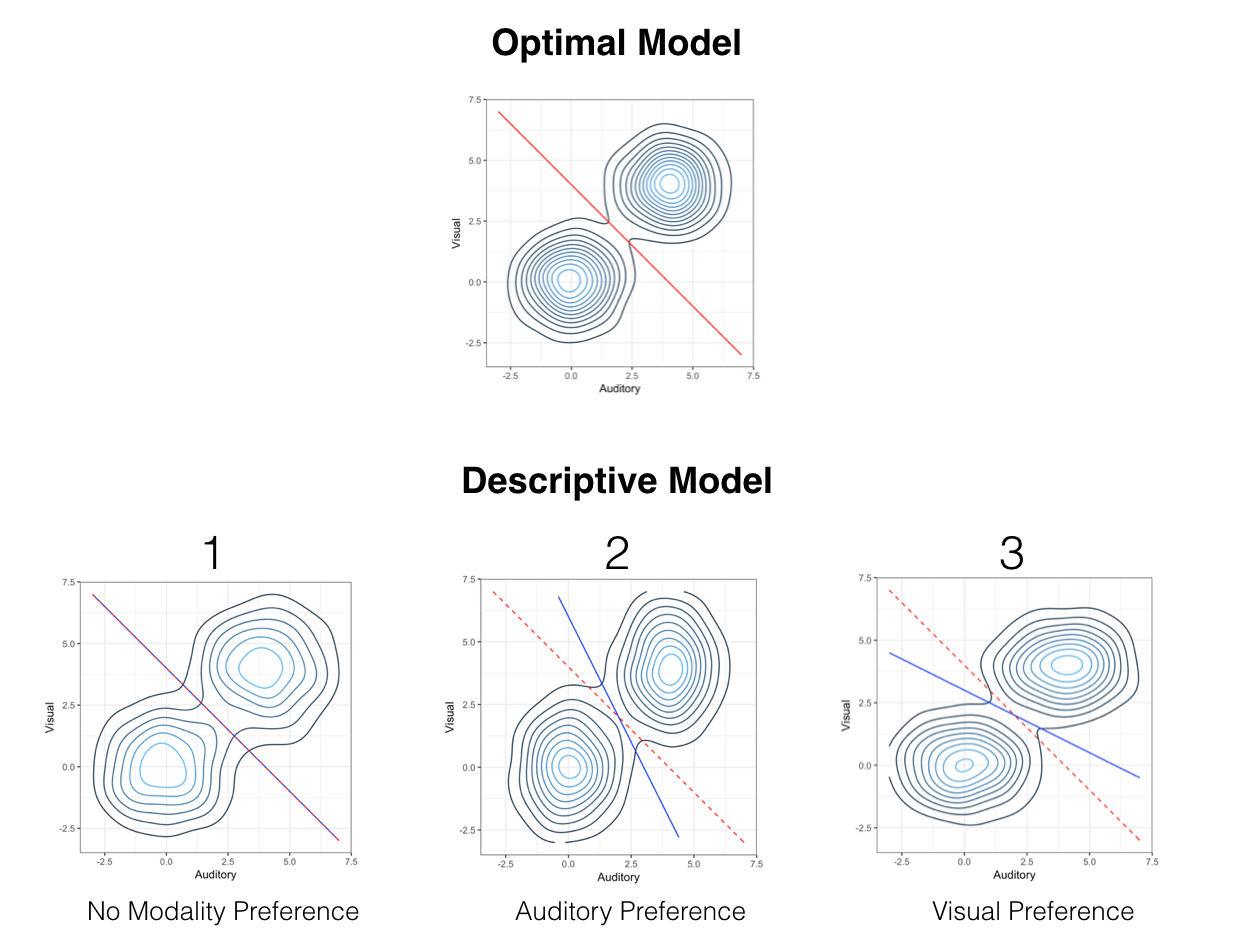
\includegraphics[width=\textwidth]{pictures/sub-optimal} \caption{Illustration using simulated data showing the example of a prediction made by the optimal model (top), and the three possible ways human participants can deviate from this prediction (bottom). These cases are the following: 1) The variance increases equally for both modalities, but the weighting scheme (characterized by the decision threshold) is optimal, 2) The auditory variance increases at a higher rate, leading to a preference for the auditory modality, and 3) The visual variance increases at a higher rate, leading to a preference for the visual modality.}\label{fig:subOptim}
\end{figure}

We compared these models to human responses in three experiments. In
Experiment 1, we studied the case where bimodal uncertainty was due to
categorical variability, only. In Experiment 2 and 3 we added auditory
and visual noise, respectively, on top of categorical variability.

\section{Experiment 1}\label{experiment-1}

In this Experiment, we test the predictions of the model in the case
where uncertainty is due to categorical variability (i.e., ambiguity in
terms of category membership) and inherent sensory noise only. We do not
add any external noise to the background. Thus, we use the following cue
weighting scheme:

\[\beta_a \propto \frac{1}{\sigma^2_{A}} = \frac{1}{\sigma^2_{A_C} + \sigma^2_{A_N}}\]
\[\beta_v \propto \frac{1}{\sigma^2_{V}} = \frac{1}{\sigma^2_{V_C} + \sigma^2_{V_N}}.\]

\subsection{Methods}\label{methods}

\subsubsection{Participants}\label{participants}

We recruited a planned sample of 100 participants from Amazon Mechanical
Turk. Only participants with US IP addresses and a task approval rate
above 85\% were allowed to participate. They were paid at an hourly rate
of \$6/hour. Participants were excluded if they reported having
experienced a technical problem of any sort during the online experiment
(N=14), or if they had less than 50\% accurate responses on the
unambiguous training trials (N=6). The final sample consisted of N = 80
participants. All participants provided informed consent before taking
the experiment.
\footnote{The sample size and exclusion criteria were specified in the pre-registration at https://osf.io/h7mzp/.}

\subsubsection{Stimuli}\label{stimuli}

For auditory stimuli, we used the continuum introduced in Vroomen,
Linden, Keetels, Gelder, and Bertelson (2004), a 9-point /aba/--/ada/
speech continuum created by varying the frequency of the second (F2)
formant in equal steps. We selected 5 equally spaced points from the
original continuum by keeping the endpoints (prototypes) 1 and 9, as
well as points 3, 5, and 7 along the continuum. For visual stimuli, we
used a cat/dog morph continuum introduced in Freedman, Riesenhuber,
Poggio, and Miller (2001). From the original 14 points, we selected 5
points as follows: we kept the item that seemed most ambiguous (point
8), the 2 preceding points (i.e., 7 and 6) and the 2 following points
(i.e., 9 and 10). The 6 and 10 points along the morph were quite
distinguishable, and we took them to be our prototypes.

\subsubsection{Design and Procedure}\label{design-and-procedure}

We told participants that an alien was naming two objects: a dog, called
\enquote{aba} in the alien language, and a cat, called \enquote{ada}. In
each trial, we presented the first object (the target) on the left side
of the screen simultaneously with the corresponding sound. For each
participant, the target was always the same (e.g., dog-/aba/). The
second sound-object pair (the test) followed on the other side of the
screen after 500ms and varied in its category membership. For both the
target and the test, visual stimuli were present for the duration of the
sound clip (\(\sim\) 800ms). We instructed participants to press
\enquote{S} for same if they thought the alien was naming another
dog-/aba/, and \enquote{D} for different if they thought the alien was
naming a cat-/ada/. We randomized the sound-object mapping (e.g.,
dog-/aba/, cat-/ada/) as well as the identity of the target (dog or cat)
across participants.

The first part of the experiment trained participants using only the
prototype pictures and the prototype sounds (12 trials, 4 each from the
bimodal, audio-only, and visual-only conditions). After completing
training, we instructed participants on the structure of the task and
encouraged them to base their answers on both the sounds and the
pictures (in the bimodal condition). There were a total of 25 possible
combinations in the bimodal condition, and 5 in each of the unimodal
conditions. Each participant saw each possible trial twice, for a total
of 70 trials/participant. Trials were blocked by condition and blocks
were presented in random order. The experiment lasted around 15
minutes.\footnote{The experiment can be accessed and played from the
  github repository: \url{https://github.com/afourtassi/WordRec/}}

\subsubsection{Model fitting details}\label{model-fitting-details}

\paragraph{Unimodal conditions}\label{unimodal-conditions}

Remember that data in these conditions allows us to derive the variances
of both the auditory and the visual categories, and that these variances
are used to make predictions about bimodal data (in the visual and
auditory baselines as well as in the optimal model). These individual
variances were derived as follows (we explain the derivation for the
auditory-only case, but the same applies for the visual-only case). We
use the same Bayesian reasoning as we did in the derivation of the
bimodal model: When presented with an audio instance \(a\), the
probability of choosing the sound category 2 (that is, to answer
\enquote{different}) is the posterior probability of this category
\(p(A_2|a)\). If we assume that both sound categories have equal
variances, the posterior probability reduces to:

\[p(A_2 | a)=\frac{1}{1+(1+b_A)\exp(\beta_{a0}+\beta_aa)}\]

with \(\beta_a=\frac{\mu_{A_1}-\mu_{A_2}}{\sigma^2_{A}}\) and
\(\beta_{a0}=\frac{\mu^2_{A_2}-\mu^2_{A_1}}{2\sigma^2_{A}}\). \(b_A\) is
the response bias in the auditory-only condition. For this model (as
well as all other models in this study), we fixed the values of the
means to be the end-points of the corresponding continuum, since these
points are the most typical instances in our stimuli. Thus, we have
\(\mu_{A1}=0\) and \(\mu_{A2}=4\) (and similarly \(\mu_{V1}=0\), and
\(\mu_{V2}=4\)). This leaves us with two free parameters: the bias
\(b_A\) and the variance \(\sigma^2_{A}\). To determine the values of
these parameters, we fit the unimodal posterior to human data in the
unimodal case.

\paragraph{Bimodal condition}\label{bimodal-condition}

In this condition, only the descriptive model is fit to the data, using
the expression of the posterior (Equation 1). Since the values of the
means are fixed, we have 3 free parameters: the variances for the visual
and the auditory modalities, respectively, and \(b\), the response bias.
The visual and auditory baselines as well as the optimal model are not
fit to the bimodal data, but their predictions are tested against these
bimodal data. All these normative models use the variances derived from
the unimodal data and the bias term derived from the fit to bimodal
data.

Although the paradigm is within-subjects, we did not have enough
statistical power to fit a different model for each individual
participant (but see Experiment 4). Instead, models were constructed
with data collapsed across all participants. The fit was done with a
nonlinear least squares regression using the NLS package in R (Bates \&
Watts, 1988). We computed the values of the parameters, as well as their
95\% confidence intervals, through non-parametric bootstrap (using 10000
iterations).

\begin{table}

\caption{\label{tab:param}Statistics for the dataset we used.}
\centering
\begin{tabular}[t]{>{\bfseries}lrrrrrrr}
\toprule
\multicolumn{1}{c}{} & \multicolumn{2}{c}{Auditory} & \multicolumn{2}{c}{Visual} & \multicolumn{3}{c}{Bimodal} \\
\cmidrule(l{2pt}r{2pt}){2-3} \cmidrule(l{2pt}r{2pt}){4-5} \cmidrule(l{2pt}r{2pt}){6-8}
Experiment & b\textsubscript{A} & Var\textsubscript{A} & b\textsubscript{V} & Var\textsubscript{V} & b\textsubscript{b} & Var\textsubscript{Ab} & Var\textsubscript{Vb}\\
\midrule
Experiment1 & 0.20 & 2.04 & 0.12 & 3.33 & 0.34 & 4.96 & 7.06\\
Experiment2 & 0.18 & 4.70 & 0.24 & 3.93 & 0.38 & 9.84 & 5.21\\
Experiment3 & 0.24 & 1.94 & -0.11 & 13.00 & 0.35 & 3.00 & 39.42\\
Experiment4 & 0.40 & 1.92 & 0.22 & 3.24 & 0.42 & 4.17 & 7.28\\
\bottomrule
\end{tabular}
\end{table}

\subsection{Results and analysis}\label{results-and-analysis}

\subsubsection{Unimodal conditions}\label{unimodal-conditions-1}

Average categorization judgments and best fits are shown in Figure
\ref{fig:unimodal}. The categorization function of the auditory
condition was slightly steeper than that of the visual condition,
meaning that participants perceived the sound tokens slightly more
categorically and with higher certainty than they did with the visual
tokens. The unimodal models' estimates are shown in Table
\ref{tab:param}.

\begin{figure}[!h]
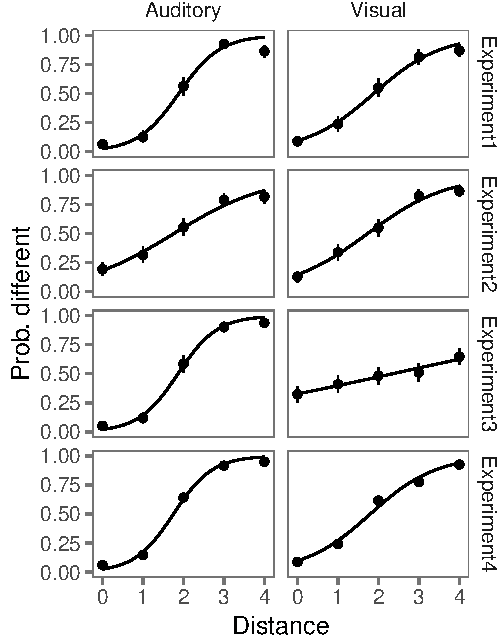
\includegraphics[width=\textwidth]{ms_files/figure-latex/unimodal-1} \caption{Human responses in the unimodal conditions across the three experiments. Points represent the proportion of `different' to `same' responses in the auditory-only condition (left), and visual-only condition (right). Error bars are 95\% confidence intervals. Solid lines represent best unimodal posterior fits.}\label{fig:unimodal}
\end{figure}

\subsubsection{Bimodal condition}\label{bimodal-condition-1}

Figure \ref{fig:bimodal} compares the predictions of the normative and
descriptive models against human responses. Remember that the normative
models use the parameters estimated from the unimodal conditions (where
people see input from only one modality) to predict behavior in the
bimodal condition (where people see input from both modalities). The
descriptive model has a similar structure than the optimal model, but is
directly fit to human responses in the bimodal condition in order to
allow us to assess deviation from optimaity.

We found, through comparing the correlation values, that the optimal
model explained more variance than the visual and auditory models did.
However, the optimal model was not perfect: It explained less variance
than the descriptive model did, which indicates a deviation from
optimality. To investigate this deviation, we compare the parameter
values of the optimal model to the values obtaied in the decriptive
model (Table
\ref{tab:param}).\footnote{Note that the descriptive model explained almost all the variance in mean responses, which makes it a reasonble proxy for human real performance in the bimodal condition.}.
We note an increase in \emph{both} the auditory and visual variances.
This increase in noise is compatible with the fact that human responses
appear to be pulled towards chance (i.e., the value O.5) when compared
to the optimal model (see \ref{fig:bimodal}). Below we investigate if
this deviation from optimality can be related to the cue combination
strategy.

\subsubsection{Cue combination}\label{cue-combination}

We analyzed if the cue combination was performed in an optimal way, or
if there was a systematic preference for one modality when making
decisions in the bimodal condition. As explained in \ref{fig:subOptim},
modality preference can be characterized formally as a deviation from
the decision threshold predicted by the optimal model. The results in
Figure \ref{fig:bias} (top) show both the decision threshold derived
from the descriptive model (in black) and the decision threshold
predicted by the optimal model (in red). We found that the descriptive
and optimal decision thresholds were almost identical. Indeed,
non-parametric resampling of the data showed no evidence of a deviation
from the optimal prediction (Figure~\ref{fig:bias}, bottom).

\begin{figure}[!h]
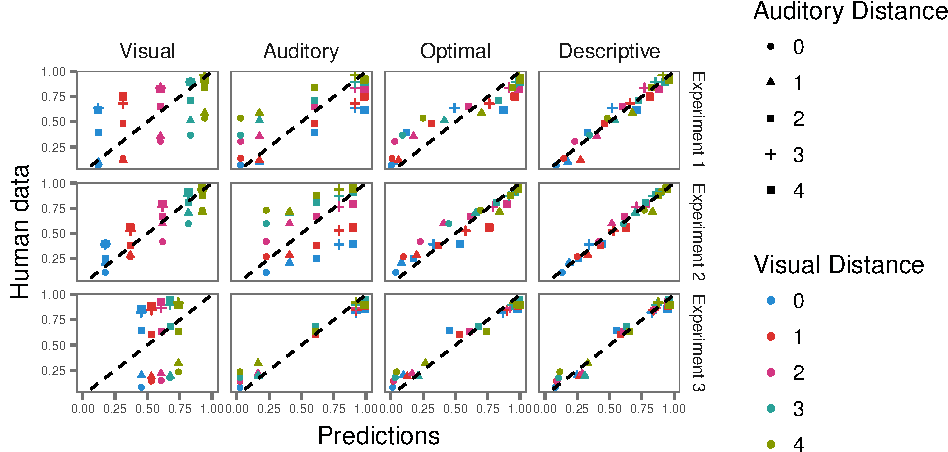
\includegraphics[width=\textwidth]{ms_files/figure-latex/bimodal-1} \caption{Human responses vs. Models' predictions in the bimodal condition across the three experiments. Each point represents data form a particular audio-visual matching (corresponding to an instance from the set of 5x5 possible matchings in the audio-visual space). Shape represents auditory distance from the target, and color represents visual distance from the target. Thus, each point is characterized by both  shape and color.}\label{fig:bimodal}
\end{figure}

\subsection{Discussion}\label{discussion}

This experiment studied the way participants combine multimodal
information to recognize novel words. We found that the optimal model
explained more variance than the auditory or the visual models did,
indicating that particiapants take into account both the auditory and
visual cues when making a decision. That said, Figure \ref{fig:bimodal}
shows that the participants deviated slightly --- but systematically---
from the optimal prediction in that they were slightly pulled toward
chance (i.e., the probability 0.5). This fact was captured by the
increase in the value of the variance associated with each modality (as
can be noted from Table \ref{tab:param}). Note, however, that despite
this increase response randomness in the bimodal condition, our analysis
of modality preference showed that the \emph{relative} values of these
variances were not different (Figure~\ref{fig:bias}), meaning that there
was no evidence for a modality preference.

To sum up, 1) the participants used both the auditory and visual
information, 2) they responded slightly more randomly that what was
predicted, but 3) this increased randomness was general and did not
influence the cue combination strategy, i.e., the participants still
weighted modalities according to their relative reliability as predicted
by the optimal model. This situation corresponds to the first case of
sub-optimality described in Figure~\ref{fig:subOptim}.

In Experiment 1, we tested word recognition when there was multimodal
uncertainty in terms of category membership and inherent perceptual
noise, only. In real life, however, both sound and visual tokens can
undergo distortions due to noisy factors in the environment (e.g., car
noise in the background, blurry vision in a foggy weather). In
Experiment 2 and 3, we explore this additional level of uncertainty.

\section{Experiment 2}\label{experiment-2}

In this Experiment, we explored the effect of added envirnonmental noise
\(\sigma^2_{E}\) on performance. We tested a case where the background
noise was added to the auditory modality. We were interested to know if
participants would treat this new source of uncertainty as predicted by
the optimal model, that is, according to the following weighting scheme:

\[\beta_a \propto \frac{1}{\sigma^2_{A}} = \frac{1}{\sigma^2_{C_A}+\sigma^2_{N_A} + \sigma^2_{E_A}}\]
\[\beta_v \propto \frac{1}{\sigma^2_{V}} = \frac{1}{\sigma^2_{C_A}+\sigma^2_{N_A}}.\]

The alternative hypothesis is that noise in one modality leads to a
systematic preference for the non-noisy modality.

\subsection{Methods}\label{methods-1}

\subsubsection{Participants}\label{participants-1}

A sample of 100 participants was recruited online through Amazon
Mechanical Turk. We used the same exclusion criteria as in Experiment 1.
7 participants were excluded because they had less than 50\% accurate
responses on the unambiguous training trials. The final sample consisted
of N = 93 participants.

\subsubsection{Stimuli and Procedure}\label{stimuli-and-procedure}

We used the same visual stimuli as in Experiment 1. We also used the
same auditory stimuli, but we convolved each item with Brown noise of
amplitude 1 using the free sound editor Audacity (2.1.2). The average
signal-to-noise ratio was - 4.4 dB. The procedure was exactly the same
as in the previous experiment, except that the test stimuli (but not the
target) were presented with the new noisy auditory stimuli.

\subsection{Results}\label{results}

The analysis are similar to the analysis we did in Experiment 1.

\subsubsection{Unimodal condition}\label{unimodal-condition}

We fit a model for each modality. Figure \ref{fig:unimodal} shows human
responses together with their best fits. The visual data is a
replication of the visual data in Experiment 1. The auditory data, in
contrast, were flatter, showing more uncertainty.

\subsubsection{Bimodal condition}\label{bimodal-condition-2}

We used the values derived from the unimodal condition to construct the
visual, auditory and optimal models. In addition, we fit a descriptive
model which allowed us to assess real human performance in this
condition. Figure \ref{fig:bimodal} shows that, similar to Experiment 1,
the optimal model explained more variance than the auditory and visual
models did (note, however, that the visual model explained more variance
than the auditory model did). Also similar to Exeperiment 1, the values
of the variances increased in the bimodal condition (Table
\ref{tab:param}).

\subsubsection{Cue combination}\label{cue-combination-1}

Here we investigated whethere the observed increase in the auditory and
visual variances affected the relative weighting of the corresponding
modalities. Figure~\ref{fig:bias} (top) shows that the participants'
decision threshold deviated from optimality, and that this deviation was
biased towards the visual modality (the non-noisy modality). Indeed
non-parametric resampling of the data showed a decrease in the value of
the slope in the descriptive model compared to the optimal model
(Figure~\ref{fig:bias}, bottom).

\subsection{Discussion}\label{discussion-1}

Experiment 2 tested audi-visual combination in the case where the
auditory input was noisy. We found, similar to Experiment 1, that the
optimal model explained more variance than the auditory or the visual
models did. In other words, despite additional noise, participants still
used information from the noisy modality to recognize words. We also
found a similar discrepancy between the descriptive and optimal models
as response randomness increased along both the auditory and the visual
modalities. As for the relative weighting, and contrary to Experiment 1
where modalities were weighted optimally, we found in this experiment
that the visual modality had a greater weight than what was expected
from its relative reliability. This situation corresponds to the second
case of sub-optimality described in Figure \ref{fig:subOptim}.

Whereas in Experiment 2 we tested the case of added background noise to
the auditory modality, in Experiment 3 we test the case of added noise
to the visual modality.

\section{Experiment 3}\label{experiment-3}

Similar to Experiment 2, we were interested to know if participants
would treat additional uncertainty as predicted by the optimal model,
that is, according to the following weighting scheme:

\[\beta_a \propto \frac{1}{\sigma^2_{A}} = \frac{1}{\sigma^2_{A_C}+\sigma^2_{A_N}}\]
\[\beta_v \propto \frac{1}{\sigma^2_{V}} = \frac{1}{\sigma^2_{V_C}+\sigma^2_{V_N} + + \sigma^2_{V_E}}.\]

The alternative hypothesis is that noise in the visual modality would
lead to a preference for the auditory input, just like noise in the
auditory modality lead to a preference for the visual input in
Experiment 2.

\subsection{Methods}\label{methods-2}

\subsubsection{Participants}\label{participants-2}

A planned sample of 100 participants was recruited online through Amazon
Mechanical Turk. We used the same exclusion criteria as in both previous
experiments. N=2 participants were excluded because they reported having
a technical problem, and N=10 participants were excluded because they
had less than 50\% accurate responses on the unambiguous training
trials. The final sample consisted of N = 88 participants.

\subsubsection{Stimuli and Procedure}\label{stimuli-and-procedure-1}

We used the same auditory stimuli as in Experiment 1. We also used the
same visual stimuli, but we blurred the tokens using the free image
editor GIMP (2.8.20). We used a Gaussian blur with a
radius\footnote{A features that modulates the intensity of the blur.} of
10 pixels. The experimental procedure was exactly the same as in the
previous Experiments.

\subsection{Results}\label{results-1}

\begin{figure}[!h]
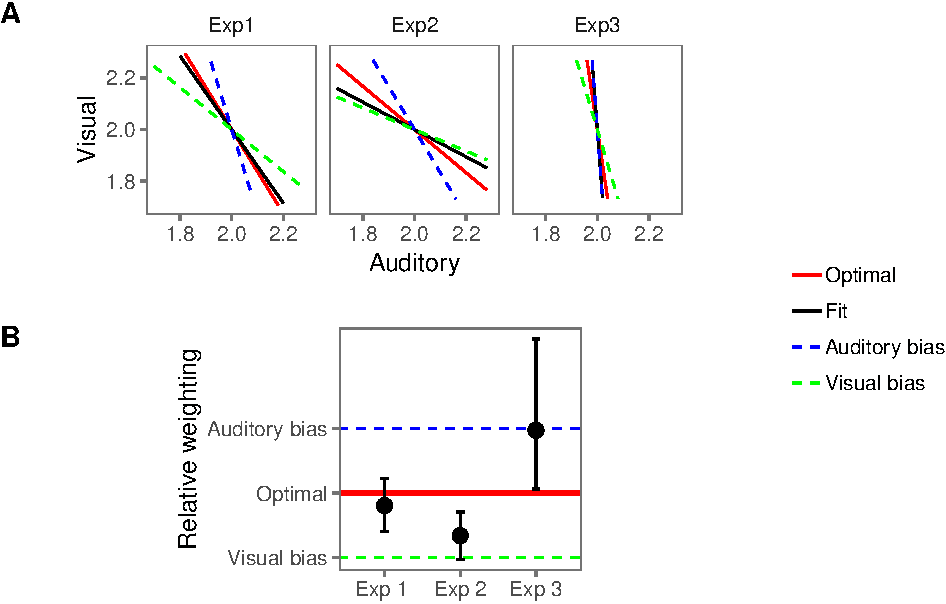
\includegraphics[width=\textwidth]{ms_files/figure-latex/bias-1} \caption{Modality preference is characterized as a deviation from the optimal decision threshold. A) The decision thresholds of both the optimal and the descriptive models (solid red and black lines, respectively). Deviation from optimality is compared to two hypothetical cases of modality preference. In these cases, deviation from  optimality is due to over-lying on the visual or the auditory input by a factor of 2 (green and blue dotted lines, respectively). B) An alternative way to represent the same data. Each point represents the value of the decision threshold's slope derived from the descriptive model relative to that of the optimal model (log-scaled). The lines represent the optimal case as well as the two hypothetical cases of modality preference. Error bars represent 95\% confidence intervals over the distribution obtained through non-parametric resampling.}\label{fig:bias}
\end{figure}

\subsubsection{Unimodal conditions}\label{unimodal-conditions-2}

Figure \ref{fig:unimodal} shows responses in the unimodal conditions as
well as the corresponding fits. The auditory data is a replication of
the auditory data in Experiment 1. As for the visual data, we found
that, in contrast to Experiment 1 and 2, responses were flatter, showing
much more uncertainty.

\subsubsection{Bimodal condition}\label{bimodal-condition-3}

Figure \ref{fig:bimodal} shows that almost all the variance was captured
by the auditory model alone, the addition of visual information in the
optomal model did not improve the prediction of human responses. Similar
to Exeperiment 1 and 2, the values of the variances increased in the
bimodal condition (Table \ref{tab:param}).

\subsubsection{Cue Combination}\label{cue-combination-2}

Figure \ref{fig:bias} indicates that the decision threshold was biased
towards the auditory modality (the non-noisy modality). Indeed
non-parametric resampling of the data showed an increase in the value of
the slope in the descriptive model compared to the optimal model
(Figure~\ref{fig:bias}).

\subsection{Discussion}\label{discussion-2}

Experiment 3 tested audi-visual combination in the case where the visual
input was noisy. Whereas in previous experiments the optimal model
explained more variance than the auditory or the visual models did, here
the auditory model alone explained almost all the variance. In other
words, though participants were sensitive to variation in the noisy
visual input when presented in isolation (as shown in Figure
\ref{fig:unimodal}), they tended to ignore this information when the
visual input was presented simultaneusel with the auditory input (i.e.,
in the bimodal condition). Instead, they relied almost exclusively on
the non-noisy auditory
modality.\footnote{The reason why we saw this (floor) effect when we added noise to the visual modality (Experiment 3), and not when we added noise to the auditory modality (Experiment 2), is the fact that our visual stimuli were originally perceived less categorically and with less certainty than the auditory stimuli (see Experiment 1 in \\ref{fig:unimodal}). This fact made it more likely for the visual categorization function to become flat and uninformative after a few drops in precision due to noise on the one had, and to the additional randomness induced by the bimodal presentation on the other hand.}

This finding corresponds to the third case of sub-optimality described
in Figure~\ref{fig:subOptim}. Indeed, precision dropped for both
modalities in the bimodal condition compared to the unimodal condition.
But the drop was much greater for the visual modality, resulting in a
much lower weight assigned to it than what is expected from the optimal
model. Therefore, just like participants over-relied on the visual
modality when the auditory modality was noisy (Experiment 2), they also
over-relied on the auditory modality when the visual modality was noisy
(Experiment 3).

So far we have studied the problem of cue combination at the population
level --- the models were fit to the data aggregated across all
participants. However, it is important to investigate individual
variability, especially in Experiment 1 where we reported optimal cue
combination. In fact, it is possible that a large part of the
participants relied primarily on the visual modality and another part on
the auditory modality. Such an extreme individual variability could
possibly lead to an aggregate beahvior which appears optimal, but such
optimality would be spurious. In order to rule out this extreme case, we
need to examine the distribution of the specific cue combibination
strategies followed by the participants.

\section{Experiment 4}\label{experiment-4}

As we noted earlier, we did not have enough statistical power to fit a
different model for each participant. Thus, in the current experiment,
we re-ran Experiment 1 while extending its length, allowing us to
collect the number of datapoints necessary to fit the models for each
participant.

\subsubsection{Participants}\label{participants-3}

We recruited a planned sample of \(N=\) 50 participants from Amazon
Mechanical Turk. Only participants with US IP addresses and a task
approval rate above 99\% were allowed to participate. They were paid at
an hourly rate of \$6/hour. Participants were excluded if they reported
having experienced a technical problem of any sort during the online
experiment (\(N=\) 0), or if they had less than 75\% accurate responses
on the unambiguous training trials (\(N=\) 7). The final sample
consisted of \(N =\) 43 participants. All participants provided informed
consent before taking the
experiment.\footnote{The sample size, exclusion criteria and the main analysese were pre-registered at https://osf.io/h7mzp/.}

\subsubsection{Stimuli}\label{stimuli-1}

We used the same stimuli as in Experiment 1.

\subsubsection{Design and Procedure}\label{design-and-procedure-1}

The design and procedure were similar to Experiment 1. There were,
however, two differences: 1) We increased the number of responses
elicited per subject from 70 to 300, and 2) we randomized the order of
the three blocks (i.e., visual-only, auditory-only, and audio-visual)
\emph{within} subject: Each participant saw the 3 blocks exactly 6
times, covering all possible ordering combinations. Unlike the
between-subjet randomzation in Experiment 1, this choices allowed us to
avoid any confounding effects due to the order of exposure.

\begin{figure}[!h]
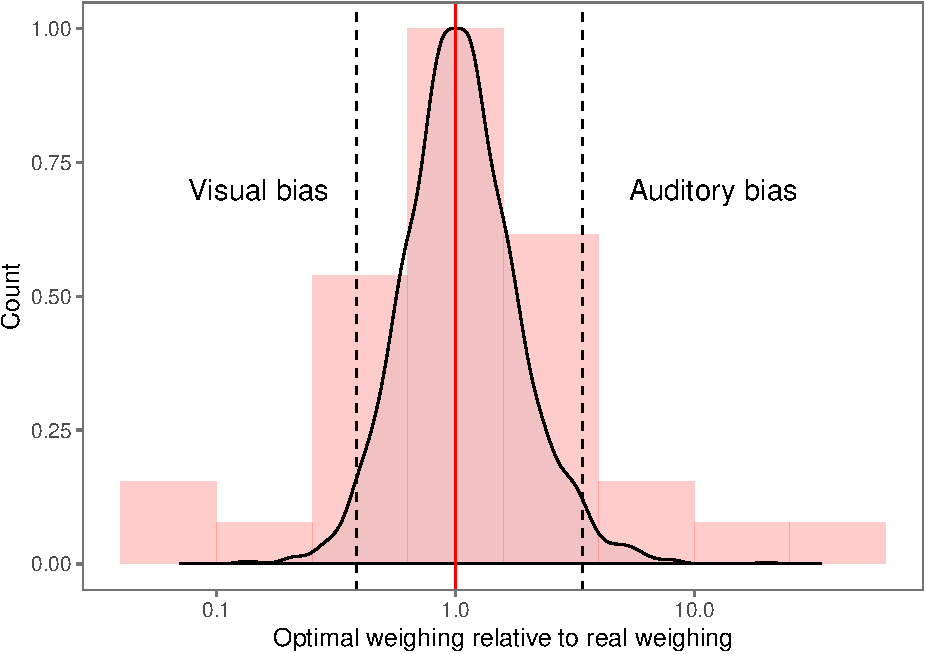
\includegraphics[width=\textwidth]{ms_files/figure-latex/weights-1} \caption{The histogram shows the distribution of the participants' optimal cue weighing  relative the observed (i.e., descriptive) cue weigting (see Figure 3). Participant are optimal when this relative value is equal to 1 (red solid line). Values larger than 1 suggest over-reliance on the auditory modality whereas values lower than 1 suggest over-reliance on the visual modality. The density plot shows the distribution of simulated individual responses from the population-level probabilistic model. The dashed lines represent 95\% confidence intreval on this simulated distribution. Participants that are outside this interval can be understood as over-relying on the auditory or visual modality in a non-random way (i.e., with p < 0.05).}\label{fig:weights}
\end{figure}

\subsection{Results}\label{results-2}

\subsubsection{Unimodal and Bimodal
conditions}\label{unimodal-and-bimodal-conditions}

In order to replicate the analysis of Experiment 1, we started by
fitting population-level models to the aggregated data. Indeed, we found
that the results --- as shown in Figure \ref{fig:unimodal}, Figure
\ref{fig:bimodal}, and Table \ref{tab:param} --- mirror closely the
patterns obtained in Experiment 1.

\subsubsection{Cue combinaton}\label{cue-combinaton}

We analyzed the cue combination strategies at the individual level. For
each participant, we computed the optimal weighing,
\(\frac{\sigma^2_{A}}{\sigma^2_{V}}\), relative to the observed (i.e.,
descriptive) weighing, \(\frac{\sigma^2_{Ab}}{\sigma^2_{Vb}}\). We show
the resulting distribution in Figure \ref{fig:weights}. We note first
that the distribution has a rather bimodal shape, centered around the
optimal cue combination strategy. This finding rules out the hypotheis
that optimality at the population level is a spurious finding, i.e.,
only obtained via aggregating over various sub-otimal strategies.

In addition, we asked whether the observed variance in the individual
distribution was due to the randomness inherent to the process of
sampling from a probabilsitic model or whether it corresponded to a real
between-subject variability induced by different cue weighing
strategies. We simulated responses through sampling from the
population-level models and we computed the resuting distribution of cue
weighing for each simulated indivudual leading to the density function
in Figure \ref{fig:weights}. We can observe that most empirical values
fall within the 95\% confidence interval of the simulated density,
showing that this part of the variance can be due to mere sampling
randomness. However, a few participants had values outide this interval,
indicating that they systematically over-relied on the visual modality
(\(N=\) 5) or the auditory modality (\(N=\) 6) with p-value\$
\textless{} 0.05\$.

\subsection{Discussion}\label{discussion-3}

This experiment was an extension to Experiment 1. Through collecting
larger-size data per subject, we were able to analyze the cue
combination optimality, not only at the population level, but also at
the individual level. The population-level analysis replicated the
results of Experiment 1. The individual-level analysis showed that the
distribution of cue combination scores had a unimodal shape centered
around the optimal combination, thus reflecting geuine cue combination
at the individual level. That said, the variance of this distribution
indicates that a few participants tended to over-rely on the auditory
modality and others tended to over-rely on the visual modality beyond
sampling errors.

\section{General Discussion}\label{general-discussion}

In the current paper, we explored word identification under uncertainty
about both words and their referents. We conducted an ideal observer
analysis of this task whereby a model provided predictions about how
information from each modality should be combined in an optimal fashion.
The predictions of the model were tested in a series of four experiments
where instances of both the form and the meaning were ambiguous with
respect to their category membership only (Experiment 1 and 4), when
instances of the form were perturbed with additional background noise
(Experiment 2), and when instances of the referent were perturbed with
additional visual noise (Experiment 3). We discuss the findings of these
studies first with respect to our ideal observer model and inferences
about optimality and second with respect to their implications for word
identification more generally.

\subsection{Patterns of optimality and
sub-optimality}\label{patterns-of-optimality-and-sub-optimality}

In all of our experiments, and when compared to the predictions of the
visual or the auditory models, participants generally relied on both
modalities to make their decisions in the bimodal condition. Indeed, in
Experiment 1 and 2, the optimal model accounted for more variance in
mean responses than the auditory or the visual models did. In Experiment
3, participants appeared to rely on one modality, but this was likely a
floor effect, due to the fact that noise made the visual input barely
perceptible. Further, in Experiment 1 and 4, which did not involve
background noise, participants not only relied on both modalities, but
generally weighted these modalities according to the predictions of the
optimal model, that is, according to their relative reliability. At the
individual level, Experiment 4 showed that most participant were
near-optimal. Only a few subjects over-relied on the auditory or visual
modalities beyond sampling errors.

More generally, the idea is that it is easier to integrate correlated,
redundant cues (e.g., the size of a an object based on both visual and
haptic information) into a unified percept, than it is to combine
perceptually uncorrelated cues to make a categorization judgement ,e.g.,
recognizing a freshly learned object category based on its distinctive
features such as shape and color. We argue that our task --- which
consists in combining perceptually uncorrelated cues from the auditory
and visual modalities to recognize a novel word --- is more similar to
the second case.

Despite this overall pattern, we documented two major cases of
sub-optimality. First, in all experiments, the variance associated with
each modality increased in the bimodal condition compared to the
unimodal conditions. Participants responded slightly more randomly in
the bimodal condition than they did in the unimodal conditions. This
finding contrasts with research on multisensory integration where
associations tend to lead to a higher precision (e.g., Ernst \& Banks,
2002). Nevertheless, research on multisensory integration has typically
dealt with a special case involving correlated, redundant multimodal
cues, e.g., determining the size of an object based on visual and haptic
information. Another possible case of multisensory integration involves
perceptually uncorrelated cues, e.g., recognizing a novel category based
on some features such as shape and color (e.g., Bankieris et al., 2017)
or, in our case, recognizing novel words cues based on phonological and
semantic cues. Perhaps it is harder to integrate uncorreated cues
because information form these cues must be encoded separately through
the decision making process. In fact, retaining two separate cues at the
same time instead of forming one unified percept (as in multisensory
integration of redundant cues), or instead of retaining only one cue (as
in the unimodal case), is likely to place extra demands on cognitive
resources, which, in turn, could cause general performance to drop.
Indeed, there is evidence that cognitive load due to divided attention
(e.g., when performing two tasks at the same time) has a detrimental
effect on word recognition (Mattys \& Wiget, 2011).

Some previous research bas found similar cases of suboptimal behavior.
For instance, studies that have explored the identification of
ambiguous, newly learned pairs of word-referent associations have
reported what appears to be a decrease in speech perception acuity in
both children (Stager \& Werker, 1997) and adults (Pajak, Creel, \&
Levy, 2016). Recently, Hofer and Levy (2017) provided a probabilistic
model of this phenomenon. In agreement with the findings of our study,
Hofer and Levy (2017) characterized the apparent reduction in perceptual
acuity as an increase in the noise variance of the auditory modality.
Our findings, besides providing more evidence to this documented fact,
suggest that the reduction in perceptual acuity may occur simultaneously
in both the auditory \emph{and} the visual modalities.

The second case of sub-optimality is related to how participants
weighted the cues from the visual and the auditory modalities in a noisy
context. In contrast to Experiment 1 adn 4 where the combination was
indistinguishable from the optimal prediction, results of Experiment 2
and 3 suggested that participants had a systematic preference for the
other (non-noisy) modality. This finding aligns with previous work that
suggests that when the auditory signal is degraded, participants
compensate by relying more on other sources of information such as the
accompanying visual cues, the semantic/syntactic context, or the
top-down expectations. This kind of compensation has been observed with
adults (Mattys et al., 2012; Tanenhaus et al., 1995), and recent
evidence suggests that it starts in childhood (K. MacDonald, Marchman,
Fernald, \& Frank, 2018; Yurovsky, Case, \& Frank, 2017). Generally
speaking, previous experimental studies have not differentiated between
an optimal compensatory strategy (i.e., relying more on the alternative
source while using all information still available in the distorted
signal), and a sub-optimal strategy (i.e., relying more on the
alternative source while ignoring at least some of the information still
available in the distorted signal), however. The formal approach
followed in this paper allowed us to tease apart these two
possibilities, and our analysis supports the sub-optimal compensatory
strategy: The preference for the non-noisy modality is above and beyond
what can be explained by the relative reliability alone, meaning that
the participants tend to ignore at least part of the information still
available in the noisy modality.

This second case of sub-optimal behavior may be related to the fact that
language understanding under degraded conditions is cognitively more
taxing than language understanding under normal conditions (Mattys et
al., 2012; Peelle, 2018; Rönnberg, Rudner, Lunner, Zekveld, \& others,
2010). Perhaps these demands lead to sub-optimal behavior (i.e.,
over-reliance on the less noisy cue) as participants seek to minimized
cognitive effort. One could also explain this phenomenon in terms of the
metacognitive experience about the fluency with which information is
processed. The perceived perceptual fluency (e.g., the ease with which a
stimulus' physical identity can be identified) can affect a wide variety
of human judgements (see Schwarz, 2004 for a review). In particular,
variables that improve fluency tend to increase liking/preference
(Reber, Winkielman, \& Schwarz, 1998). In our case, the subjective
experience of lower fluency in the noisy modality might cause people to
underestimate information that can be extracted from this modality,
especially when presented simultaneously with a higher fluency
alternative.

\subsection{Word recognition in the
wild}\label{word-recognition-in-the-wild}

An important question to ask is how the combination mechanism --- as
revealed in our controlled study --- scales up to real life situations.
Note that in order to test audio-visual cue combination under
uncertainty, we had to use a case of double ambiguity, that is, a case
where both the word forms (\enquote{ada}--\enquote{aba}) and the
referents (cat--dog) were similar and, thus, confusable. However, to
what extent does such a case occur in real languages? Cross-linguistic
corpus analyses suggest that lexical encoding tends, surprisingly,
towards double ambiguity in many languages (Dautriche, Mahowald, Gibson,
\& Piantadosi, 2017; Monaghan, Shillcock, Christiansen, \& Kirby, 2014;
Tamariz, 2008). For instance, Dautriche et al. (2017) analyzed 100
languages and found that words that are similar phonologically tend to
be similar semantically as well. These studies suggest that the case of
double uncertainty, though perhaps not pervasive, could be a real issue
in language as it increase the probability of confusability for many
words. That said, the inferences discussed here might play a more
significant role in naturalistic language comprehension when ambiguity
in both the form and/or the referent is induced by an \emph{external}
noisy context --- e.g., a very noisy party or a far away referent ---
even when these forms and referents are not confusable in normal
situations.

Though we only studied adult performance in this paper, the problem of
word recognition under uncertainty is likely more pressing for children.
In fact, children have greater difficulties differentiating the meanings
of novel similar-sounding words (e.g., \enquote{bin} vs. \enquote{din}),
even when these words are uttered very clearly (Creel, 2012; Merriman \&
Schuster, 1991; Stager \& Werker, 1997; Swingley, 2016; White \& Morgan,
2008). Such similar-sounding words can be shown to be differentiated by
infants in simplified experimental settings (e.g., Yoshida, Fennell,
Swingley, \& Werker, 2009). Nevertheless, Swingley (2007) suggested that
the ability to make this differentiation is likely not mature in early
childhood; children's representations are almost certainly noisier than
the adults' representations and may also be encoded with lower
confidence. Thus, children even more than adults might benefit from
additional disambiguating cues during new word-referent encoding and
recognition.

A multi-modal cue combination strategy might help children not only
recognize words, but also refine their underlying phonological and
semantic representations in the process. Previous research in early word
learning has -- whether implicitly or explicitly -- largely treated the
process of refining the word form and of refining the word meaning as
following a linear timeline. However, developmental data reveal that
children do not wait to have complete acquisition of word forms before
they start learning their meanings (Bergelson \& Swingley, 2012; Tincoff
\& Jusczyk, 1999). Rather, both form and meaning representations develop
in a parallel fashion. A few studies have already suggested the
possibility of an interaction between sound and meaning in early
acquisition. For instance, Waxman and Markow (1995) showed that labeling
various objects with the same name helps infants form the underlying
semantic category (but see Sloutsky \& Napolitano, 2003). And in the
opposite direction, Yeung and Werker (2009) showed that pairing similar
sounds with different objects can helps infants enhance their
sensitivity to subtle phonological contrasts in their native language.
The present study proposes a first step towards a formal framework where
these sorts of sound-meaning interactions in development can be unified
and further explored.

One salient limitation of our current work is that we used a restricted
and highly simplified stimulus set. For the auditory modality, we used
speech categories that varied along a single acoustic dimension. While
this dimension might be sufficient to recognize words in our specific
case, in general the speech signal is far more complex, varying along
several acoustic/phonetic dimensions. Additionally, these dimensions may
be highly variable due to various kinds of speaker and context
differences.

As for the visual modality, simulating meaningful variability is a more
difficult task. Indeed, parameterizing the semantic space has been a
notoriously hard problem and thus requires more simplifying assumptions.
Following previous studies (Freedman et al., 2001; Havy \& Waxman, 2016;
Sloutsky \& Fisher, 2004), we used a visual continuum along a
one-dimensional morph. This choice was motivated by the need to
construct a multimodal input where the auditory and visual components
are parametrized in a symmetrical fashion, allowing us to compare graded
effects of auditory and visual information on categorical judgment.
Though such a visual variability is clearly artificial (one does not
encounters in real life an animal that is, e.g., 30 \% dog and 70 \%
cat), we assume that the induced uncertainty form this visual stimuli
has a similar effect on word recognition as the uncertainty induced by
more naturalistic semantic variability.

It is an open question whether people use the same strategy in
controlled laboratory conditions and more naturalistic settings where
they have to deal with various levels of variability. An answer to this
question is likely to involve a multifaceted research approach that goes
beyond controlled experimentation. We believe that one fruitful approach
is to test computational mechanisms with an input that more accurately
represents the full extent of multimodal variability in the learning
environment (Dupoux, 2018; Fourtassi, Schatz, Varadarajan, \& Dupoux,
2014; Harwath, Torralba, \& Glass, 2016; B. C. Roy, Frank, DeCamp, \&
Roy, 2015).

\section{Conclusions}\label{conclusions}

Our work provides a formal framework where old and new questions about
word recognition as well as other categorical tasks involving
uncorrelated cues can be given a precise formulation. We used a novel
method which enabled us not only to test for optimality as in prevous
studies (e.g., Bankieris et al., 2017; Bejjanki et al., 2011), but also
to examine systamtically how and by how much people deviate from
optimality in their combination strategies. This exploration is
important bla bla Rahnev and Denison (2018)

While we focused on the case of arbitrary associations in novel word
recognition, it is possible to use the same framework to study, for
instance, the case of \textit{iconicity}, that is, when there is a
resemblance between the sound of a word and its referent. Previous work
has suggested that iconicity, among other things, helps with learning
(and generalizing the meaning of) new words (see Dingemanse, Blasi,
Lupyan, Christiansen, \& Monaghan, 2015 for a review). Using the
research strategy in this paper, we can, for example, test whether
iconicity has such an advantage because it mitigates the sub-optimal
patterns observed with more arbitrary pairings.

Finally, though the current framework only characterizes adult word
recognition, it provides a first step towards a model where
developmental questions can also be investigated. For instance, future
work should explore whether children, like adults, use probabilistic
cues from both the auditory and the visual input to recognize ambiguous
words, the extent to which they combine these cues in an optimal
fashion, and whether this cue combination help them to refine their
early phonological and semantic representations.

\vspace{1em}

\fbox{\parbox[b][][c]{14cm}{\centering All data and code for these analyses are available at\ \url{https://github.com/afourtassi/WordRec}}}
\vspace{1em}

\section{Acknowledgements}\label{acknowledgements}

This work was supported by a post-doctoral grant from the Fyssen
Foundation.

\section{Disclosure statement}\label{disclosure-statement}

None of the authors have any financial interest or a conflict of
interest regarding this work and this submission.

\section{Appendix 1: derivation of the posterior (Equation
1)}\label{appendix-1-derivation-of-the-posterior-equation-1}

For an ideal observer, the probability of choosing category 2 when
presented with an audio-visual instance \(w = (a, v)\) is the posterior
probability of this category:

\[p(W_2 | w)=\frac{p(w|W_2)p(W_2)}{p(w|W_2)p(W_2)+p(w|W_1)p(W_1)}\]

Which reduces to:

\[p(W_2 | w)=\frac{1}{1+\frac{p(w|W_1)}{p(w|W_2)} \frac{p(W_1)}{p(W_2)}}\]
In order to further simplify the quantity \(\frac{p(w|W_1)}{p(w|W_2)}\),
we use our assumption that the cues are uncorrelated:
\[p(w | W) = p(a,v| W) = p(a| A)p(v| V)\] Using the \(\log\)
transformation, we get:

\[ \ln(\frac{p(w |W_1)}{p(w|W_2)})=\ln(\frac{p(a|W_1)}{p(a|W_2)})+\ln(\frac{p(v|W_1)}{p(v|W_2)}) \]
Under the assumption that the categories are normally distributed and
that, within each modality, the categories have equal variances, we get
(after simplification):

\[\ln(\frac{p(a|W_1)}{p(a|W_2)})=\frac{\mu_{A1}-\mu_{A2}}{\sigma^2_{A}}\times a+ \frac{\mu^2_{A2}-\mu^2_{A1}}{2\sigma^2_{A}}\]

and similarly:

\[\ln(\frac{p(v|W_1)}{p(v|W_2)})=\frac{\mu_{V1}-\mu_{V2}}{\sigma^2_{V}}\times v+ \frac{\mu^2_{V2}-\mu^2_{V1}}{2\sigma^2_{V}}\]

When putting all these terms together, we obtain this final expression
for the posterior:
\[p(W_2 | w)=\frac{1}{1+(1+b)\exp(\beta_0+\beta_aa+\beta_vv)}\]

where

\[1+b=\frac{p(W_1)}{p(W_2)}\]
\[\beta_0=\frac{\mu^2_{A2}-\mu^2_{A1}}{2\sigma^2_{A}}+\frac{\mu^2_{V2}-\mu^2_{V1}}{2\sigma^2_{V}}\]

\[\beta_a=\frac{\mu_{A1}-\mu_{A2}}{\sigma^2_{A}}\]
\[\beta_v=\frac{\mu_{V1}-\mu_{V2}}{\sigma^2_{V}}.\]

\section{References}\label{references}

\setlength{\parindent}{-0.5in} \setlength{\leftskip}{0.5in}

\hypertarget{refs}{}
\hypertarget{ref-anderson90}{}
Anderson, J. R. (1990). \emph{The adaptive character of thought}.
Hillsdale, NJ: Erlbaum.

\hypertarget{ref-Bankieris17}{}
Bankieris, K. R., Bejjanki, V., \& Aslin, R. N. (2017). Sensory
cue-combination in the context of newly learned categories.
\emph{Scientific Reports}, \emph{7}(1), 10890.

\hypertarget{ref-bates88}{}
Bates, D., \& Watts, D. (1988). \emph{Nonlinear regression analysis and
its applications}. Wiley.

\hypertarget{ref-bejjanki2011}{}
Bejjanki, V., Clayards, M., Knill, D., \& Aslin, R. (2011). Cue
integration in categorical tasks: Insights from audio-visual speech
perception. \emph{PLoS ONE}, \emph{6}.

\hypertarget{ref-bergelson2012}{}
Bergelson, E., \& Swingley, D. (2012). At 6 to 9 months, human infants
know the meanings of many common nouns. \emph{Proceedings of the
National Academy of Sciences}, \emph{109}(9).

\hypertarget{ref-Campbell2008}{}
Campbell, R. (2008). The processing of audio-visual speech: Empirical
and neural bases. \emph{Philosophical Transactions of the Royal Society
of London B: Biological Sciences}, \emph{363}(1493), 1001--1010.

\hypertarget{ref-chater06}{}
Chater, N., \& Manning, C. D. (2006). Probabilistic models of language
processing and acquisition. \emph{Trends in Cognitive Sciences},
\emph{10}, 335--344.

\hypertarget{ref-clayard08}{}
Clayards, M., Tanenhaus, M., Aslin, R., \& Jacobs, R. (2008). Perception
of speech reflects optimal use of probabilistic speech cues.
\emph{Cognition}, \emph{108}.

\hypertarget{ref-Creel2012}{}
Creel, S. (2012). Phonological similarity and mutual exclusivity:
On-line recognition of atypical pronunciations in 3--5-year-olds.
\emph{Developmental Science}, \emph{15}(5), 697--713.

\hypertarget{ref-dautriche17}{}
Dautriche, I., Mahowald, K., Gibson, E., \& Piantadosi, S. (2017).
Wordform similarity increases with semantic similarity: An analysis of
100 languages. \emph{Cognitive Science}, \emph{41}(8), 2149--2169.

\hypertarget{ref-dingemanse2015}{}
Dingemanse, M., Blasi, D. E., Lupyan, G., Christiansen, M. H., \&
Monaghan, P. (2015). Arbitrariness, iconicity, and systematicity in
language. \emph{Trends in Cognitive Sciences}, \emph{19}(10), 603--615.

\hypertarget{ref-dupoux2018}{}
Dupoux, E. (2018). Cognitive science in the era of artificial
intelligence: A roadmap for reverse-engineering the infant
language-learner. \emph{Cognition}, \emph{173}, 43--59.

\hypertarget{ref-Eberhard1995}{}
Eberhard, K., Spivey-Knowlton, M. J., Sedivy, J. C., \& Tanenhaus, M.
(1995). Eye movements as a window into real-time spoken language
comprehension in natural contexts. \emph{Journal of Psycholinguistic
Research}, \emph{24}(6), 409--436.

\hypertarget{ref-edmiston2015}{}
Edmiston, P., \& Lupyan, G. (2015). What makes words special? Words as
unmotivated cues. \emph{Cognition}, \emph{143}, 93--100.

\hypertarget{ref-ernst02}{}
Ernst, M. O., \& Banks, M. S. (2002). Humans integrate visual and haptic
information in a statistically optimal fashion. \emph{Nature},
\emph{415}(6870), 429--433.

\hypertarget{ref-feldman2009}{}
Feldman, N., Griffiths, T., \& Morgan, J. (2009). The influence of
categories on perception: Explaining the perceptual magnet effect as
optimal statistical inference. \emph{Psychological Review},
\emph{116}(4), 752--782.

\hypertarget{ref-fourtassi2014b}{}
Fourtassi, A., Schatz, T., Varadarajan, B., \& Dupoux, E. (2014).
Exploring the relative role of bottom-up and top-down information in
phoneme learning. In \emph{Proceedings of the 52nd annual meeting of the
association for computational linguistics (volume 2: Short papers)}
(Vol. 2, pp. 1--6).

\hypertarget{ref-freedman2001}{}
Freedman, D., Riesenhuber, M., Poggio, T., \& Miller, E. and. (2001).
Categorical representation of visual stimuli in the primate prefrontal
cortex. \emph{Science}, \emph{291}.

\hypertarget{ref-Geisler2003}{}
Geisler, W. S. (2003). Ideal observer analysis. In \emph{The visual
neurosciences} (pp. 825--837). Cambridge, MA: MIT Press.

\hypertarget{ref-greenberg1957}{}
Greenberg, J. (1957). \emph{Essays in linguistics}. Chicago: University
of Chicago Press.

\hypertarget{ref-harwath2016}{}
Harwath, D., Torralba, A., \& Glass, J. (2016). Unsupervised learning of
spoken language with visual context. In \emph{Advances in neural
information processing systems} (pp. 1858--1866).

\hypertarget{ref-havy2016}{}
Havy, M., \& Waxman, S. (2016). Naming influences 9-month-olds'
identification of discrete categories along a perceptual continuum.
\emph{Cognition}, \emph{156}, 41--51.

\hypertarget{ref-hillenbrand1995}{}
Hillenbrand, J., Getty, L. A., Clark, M. J., \& Wheeler, K. (1995).
Acoustic characteristics of american english vowels. \emph{Journal of
the Acoustical Society of America}, \emph{97}.

\hypertarget{ref-hofer2017}{}
Hofer, M., \& Levy, R. (2017). Modeling Sources of Uncertainty in Spoken
Word Learning. In \emph{Proceedings of the 39th Annual Meeting of the
Cognitive Science Society}.

\hypertarget{ref-kleinschmidt2015}{}
Kleinschmidt, D. F., \& Jaeger, T. F. (2015). Robust speech perception:
Recognize the familiar, generalize to the similar, and adapt to the
novel. \emph{Psychological Review}, \emph{148}.

\hypertarget{ref-Knill04}{}
Knill, D., \& Pouget, A. (2004). The bayesian brain: The role of
uncertainty in neural coding and computation. \emph{Trends in
Neurosciences}, \emph{27}(12), 712--719.

\hypertarget{ref-kuhl1991}{}
Kuhl, P. K. (1991). Human adults and human infants show a ``perceptual
magnet effect'' for the prototypes of speech categories, monkeys do not.
\emph{Perception \& Psychophysics}, \emph{50}(2), 93--107.

\hypertarget{ref-lupyan2012}{}
Lupyan, G., \& Thompson-Schill, S. L. (2012). The evocative power of
words: Activation of concepts by verbal and nonverbal means.
\emph{Journal of Experimental Psychology: General}, \emph{141}(1), 170.

\hypertarget{ref-macdonald2018}{}
MacDonald, K., Marchman, V., Fernald, A., \& Frank, M. C. (2018). Adults
and preschoolers seek visual information to support language
comprehension in noisy environments. In \emph{Proceedings of the 40th
Annual Conference of the Cognitive Science Society}.

\hypertarget{ref-marr1982}{}
Marr, D. (1982). \emph{Vision}. WH Freeman.

\hypertarget{ref-mattys11}{}
Mattys, S. L., \& Wiget, L. (2011). Effects of cognitive load on speech
recognition. \emph{Journal of Memory and Language}, \emph{65}(2),
145--160.

\hypertarget{ref-mattys12}{}
Mattys, S. L., Davis, M. H., Bradlow, A. R., \& Scott, S. K. (2012).
Speech recognition in adverse conditions: A review. \emph{Language and
Cognitive Processes}, \emph{27}(7-8), 953--978.

\hypertarget{ref-mcgurk1976}{}
McGurk, H., \& MacDonald, J. (1976). Hearing lips and seeing voices.
\emph{Nature}, \emph{264}, 746--748.

\hypertarget{ref-medina2011}{}
Medina, T., Snedeker, J., Trueswell, J., \& Gleitman, L. (2011). How
words can and cannot be learned by observation. \emph{Proceedings of the
National Academy of Sciences}, \emph{108}(22), 9014.

\hypertarget{ref-Merriman91}{}
Merriman, W., \& Schuster, J. (1991). Young children's disambiguation of
object name reference. \emph{Child Development}, \emph{62}(6),
1288--1301.

\hypertarget{ref-Monaghan2014}{}
Monaghan, P., Shillcock, R. C., Christiansen, M. H., \& Kirby, S.
(2014). How arbitrary is language? \emph{Philosophical Transactions of
the Royal Society of London B: Biological Sciences}, \emph{369}(1651).

\hypertarget{ref-Norris08}{}
Norris, D., \& McQueen, J. M. (2008). Shortlist B: A bayesian model of
continuous speech recognition. \emph{Psychological Review},
\emph{115}(2), 357--395.

\hypertarget{ref-pajak2016}{}
Pajak, B., Creel, S., \& Levy, R. (2016). Difficulty in learning
similar-sounding words: A developmental stage or a general property of
learning? \emph{Journal of Experimental Psychology: Learning, Memory,
and Cognition}, \emph{42}(9).

\hypertarget{ref-peelle2018}{}
Peelle, J. E. (2018). Listening effort: How the cognitive consequences
of acoustic challenge are reflected in brain and behavior. \emph{Ear and
Hearing}, \emph{39}(2), 204.

\hypertarget{ref-pinker1989}{}
Pinker, S. (1989). \emph{Learnability and cognition: The acquisition of
argument structure}. Cambridge, MA: MIT press.

\hypertarget{ref-rahnev2018}{}
Rahnev, D., \& Denison, R. N. (2018). Suboptimality in perceptual
decision making. \emph{Behavioral and Brain Sciences}, 1--107.

\hypertarget{ref-reber98}{}
Reber, R., Winkielman, P., \& Schwarz, N. (1998). Effects of perceptual
fluency on affective judgments. \emph{Psychological Science},
\emph{9}(1), 45--48.

\hypertarget{ref-robinson2010}{}
Robinson, C. W., \& Sloutsky, V. (2010). Development of cross-modal
processing. \emph{Wiley Interdisciplinary Reviews: Cognitive Science},
\emph{1}.

\hypertarget{ref-roy2015}{}
Roy, B. C., Frank, M. C., DeCamp, M., P., \& Roy, D. (2015). Predicting
the birth of a spoken word. \emph{Proceedings of the National Academy of
Sciences}, \emph{112}.

\hypertarget{ref-ronnberg2010}{}
Rönnberg, J., Rudner, M., Lunner, T., Zekveld, A. A., \& others. (2010).
When cognition kicks in: Working memory and speech understanding in
noise. \emph{Noise and Health}, \emph{12}(49), 263.

\hypertarget{ref-saussure1916}{}
Saussure, F. (1916). \emph{Course in general linguistics.} New York:
McGraw-Hill.

\hypertarget{ref-schwarz2004}{}
Schwarz, N. (2004). Metacognitive experiences in consumer judgment and
decision making. \emph{Journal of Consumer Psychology}, \emph{14}(4),
332--348.

\hypertarget{ref-sloutsky2004}{}
Sloutsky, V., \& Fisher, A. V. (2004). Induction and categorization in
young children: A similarity-based model. \emph{Journal of Experimental
Psychology: General}, \emph{133}(2), 166.

\hypertarget{ref-sloutsky2003}{}
Sloutsky, V., \& Napolitano, A. (2003). Is a picture worth a thousand
words? Preference for auditory modality in young children. \emph{Child
Development}, \emph{74}.

\hypertarget{ref-smith08}{}
Smith, L. B., \& Yu, C. (2008). Infants rapidly learn word-referent
mappings via cross-situational statistics. \emph{Cognition},
\emph{106}(3), 1558--1568.

\hypertarget{ref-spivey2002}{}
Spivey, M. J., Tanenhaus, M., Eberhard, K., \& Sedivy, J. C. (2002). Eye
movements and spoken language comprehension: Effects of visual context
on syntactic ambiguity resolution. \emph{Cognitive Psychology},
\emph{45}(4), 447--481.

\hypertarget{ref-stager1997}{}
Stager, C. L., \& Werker, J. F. (1997). Infants listen for more phonetic
detail in speech perception than in word-learning tasks. \emph{Nature},
\emph{388}(6640).

\hypertarget{ref-suanda2014}{}
Suanda, S. H., Mugwanya, N., \& Namy, L. L. (2014). Cross-situational
statistical word learning in young children. \emph{Journal of
Experimental Child Psychology}, \emph{126}.

\hypertarget{ref-Swingley2007}{}
Swingley, D. (2007). Lexical exposure and word-form encoding in
1.5-year-olds. \emph{Developmental Psychology}, \emph{43}(2), 454--464.

\hypertarget{ref-Swingley2016}{}
Swingley, D. (2016). Two-year-olds interpret novel phonological
neighbors as familiar words. \emph{Developmental Psychology},
\emph{52}(7), 1011--1023.

\hypertarget{ref-Tamariz2008}{}
Tamariz, M. (2008). Exploring systematicity between phonological and
context-cooccurrence representations of the mental lexicon. \emph{The
Mental Lexicon}, \emph{3}(2).

\hypertarget{ref-Tanenhaus1995}{}
Tanenhaus, M., Spivey-Knowlton, M., Eberhard, K., \& Sedivy, J. (1995).
Integration of visual and linguistic information in spoken language
comprehension. \emph{Science}, \emph{268}(5217), 1632--1634.

\hypertarget{ref-tenenbaum11}{}
Tenenbaum, J., Kemp, C., Griffiths, T., \& Goodman, N. (2011). How to
grow a mind: Statistics, structure, and abstraction. \emph{Science},
\emph{331}(6022), 1279--1285.

\hypertarget{ref-tincoff1999}{}
Tincoff, R., \& Jusczyk, P. W. (1999). Some beginnings of word
comprehension in 6-month-olds. \emph{Psychological Science},
\emph{10}(2), 172--175.

\hypertarget{ref-vlach2013}{}
Vlach, H. A., \& Johnson, S. P. (2013). Memory constraints on infants'
cross-situational statistical learning. \emph{Cognition}, \emph{127}.

\hypertarget{ref-vouloumanos2008}{}
Vouloumanos, A. (2008). Fine-grained sensitivity to statistical
information in adult word learning. \emph{Cognition}, \emph{107}(2),
729--742.

\hypertarget{ref-vouloumanos2014}{}
Vouloumanos, A., \& Waxman, S. (2014). Listen up! Speech is for thinking
during infancy. \emph{Trends in Cognitive Sciences}, \emph{18}(12),
642--646.

\hypertarget{ref-vroomen2004}{}
Vroomen, J., Linden, S. van, Keetels, M., Gelder, B. de, \& Bertelson,
P. (2004). Selective adaptation and recalibration of auditory speech by
lipread information: Dissipation. \emph{Speech Communication},
\emph{44}.

\hypertarget{ref-waxman2009}{}
Waxman, S., \& Gelman, S. (2009). Early word-learning entails reference,
not merely associations. \emph{Trends in Cognitive Sciences},
\emph{13}(6).

\hypertarget{ref-waxman1995}{}
Waxman, S., \& Markow, D. (1995). Words as invitations to form
categories: Evidence from 12-to 13-month-old infants. \emph{Cognitive
Psychology}, \emph{29}(3), 257--302.

\hypertarget{ref-white2008b}{}
White, K., \& Morgan, J. (2008). Sub-segmental detail in early lexical
representations. \emph{Journal of Memory and Language}, \emph{59}.

\hypertarget{ref-yeung09}{}
Yeung, H., \& Werker, J. (2009). Learning words' sounds before learning
how words sound: 9-month-olds use distinct objects as cues to categorize
speech information. \emph{Cognition}, \emph{113}, 234--243.

\hypertarget{ref-yoshida2009}{}
Yoshida, K., Fennell, C., Swingley, D., \& Werker, J. (2009).
14-month-olds learn similar-sounding words. \emph{Developmental
Science}, \emph{12}.

\hypertarget{ref-yurovsky2015}{}
Yurovsky, D., \& Frank, M. C. (2015). An Integrative Account of
Constraints on Cross-Situational Learning. \emph{Cognition}, \emph{145}.

\hypertarget{ref-yurovsky2017}{}
Yurovsky, D., Case, S., \& Frank, M. C. (2017). Preschoolers flexibly
adapt to linguistic input in a noisy channel. \emph{Psychological
Science}, \emph{28}(1), 132--140.


\end{document}
